%%% Exemplo de utilizacao da classe ITA
%%%
%%%   por        Fabio Fagundes Silveira   -  ffs [at] ita [dot] br
%%%              Benedito C. O. Maciel     -  bcmaciel [at] ita [dot] br
%%%              Giovani Volnei Meinertz   -  giovani [at] ita [dot] br
%%%    	         Hudson Alberto Bode       -  bode [at] ita [dot]br
%%%    	         P. I. Braga de Queiroz    -  pi [at] ita [dot] br
%%%    	         Jorge A. B. Gripp         -  gripp [at] ita [dot] br
%%%    	         Juliano Monte-Mor         -  jamontemor [at] yahoo [dot] com [dot] br
%%%    	         Tarcisio A. B. Gripp      -  tarcisio.gripp [at] gmail [dot] com
%%%    	         
%%%
%%%  IMPORTANTE: O texto contido neste exemplo nao significa absolutamente nada.  :-)
%%%              respectivas utilizacoes.
%%%
%%%  Tese.tex  2016-08-25
%%%  HeadURL: http://www.apgita.org.br/apgita/teses-e-latex.php
%%%
%%% ITALUS
%%% Instituto Tecnologico de Aeronautica --- ITA, Sao Jose dos Campos, Brasil
%%%                   http://groups.yahoo.com/group/italus/
%%% Discussion list: italus {at} yahoogroups.com
%%%
%++++++++++++++++++++++++++++++++++++++++++++++++++++++++++++++++++++++++++++++
% Para alterar o TIPO DE DOCUMENTO, preencher a linha abaixo \documentclass[?]{?}
%   \documentclass[tg]{ita}			= Trabalho de Graduacao
%   \documentclass[tgfem]{ita}	= Para Engenheiras
%   								msc     		= Dissertacao de Mestrado
%   								mscfem   		= Para Mestras
%   								dsc      		= Tese de Doutorado
%   								dscfem   		= Para Doutoras
%   								quali    		= Exame de Qualificacao
%   								qualifem 		= Exame de Qualificacao para Doutoras
% Para 'Draft Version'/'Versao Preliminar' com data no rodape, adicionar 'dv':
%   \documentclass[dsc, dv]{ita} 
% Para trabalhos em Ingles, adicionar 'eng':
%   \documentclass[dsc, eng]{ita}
%		\documentclass[dsc, eng, dv]{ita}
%++++++++++++++++++++++++++++++++++++++++++++++++++++++++++++++++++++++++++++++
\documentclass[tg, eng]{ita}    % ITA.cls based on standard book.cls 
% Quando alterar a classe, por exemplo de [msc] para [msc, eng]) rode mais uma vez o botao BUILD OUTPUT caso haja erro
\usepackage{ae}
\usepackage{graphicx}
\usepackage{epsfig}
\usepackage{amsmath}
\usepackage{amssymb} 
%\usepackage{subfig}
\usepackage{multirow}
\usepackage{float}
\usepackage{subcaption}
\usepackage[ruled]{algorithm2e}
\usepackage{textcomp}
\usepackage[latin1]{inputenc}

%++++++++++++++++++++++++++++++++++++++++++++++++++++++++++++++++++++++++++++++
% Espacamento padrao de todo o documento
%++++++++++++++++++++++++++++++++++++++++++++++++++++++++++++++++++++++++++++++
\onehalfspacing

%singlespacing Para um espacamento simples
%onehalfspacing Para um espacamento de 1,5
%doublespacing Para um espacamento duplo


%++++++++++++++++++++++++++++++++++++++++++++++++++++++++++++++++++++++++++++++
% Identificacoes (se o trabalho for em ingles, insira os dados em ingles)
% Para entradas abreviadas de Professora (Profa.) em portugues escreva: Prof$^\textnormal{a}$.
%++++++++++++++++++++++++++++++++++++++++++++++++++++++++++++++++++++++++++++++
\course{Electronics Engineering} % Programa de PG ou Curso de Graduacao
%\area{Sistemas Aeroespaciais e Mecatronica} % area de concentracao na PG (Nao utilizado no caso de TG)

% Autor do trabalho: Nome Sobrenome
\authorgender{masc}                     %sexo: masc ou fem
\author{Luis Guilherme Gomes}{Aguiar}
\itaauthoraddress{Rua H8A, 131}{12228-460}{S\~ao Jos\'e dos Campos--SP}

% Titulo da Tese/Dissertacao
\title{Simulated Humanoid Robot Control with Reinforcement Learning}

% Orientador
\advisorgender{masc}                    % masc ou fem
\advisor{Prof. Dr.}{Marcos Ricardo Omena de A. M\'aximo}{ITA}


% Coorientador (Caso nao haja coorientador, colocar ambas as variaveis \coadvisorgender e \coadvisor comentadas, com um % na frente)
\coadvisorgender{masc}									% masc ou fem
\coadvisor{Prof. Dr.}{Takashi Yoneyama}{ITA}
% Pro-reitor da Pos-graduacao

%Coordenador do curso no caso de TG
%\bosscoursegender{masc}									% masc ou fem
%\bosscourse{Prof.~Dr.}{John Walker}

%Coordenador do curso no caso de TG
\bosscoursegender{masc}									% masc ou fem
\bosscourse{Prof.~Dr.}{Roberto Kawakami Harrop Galv\~ao}

% Palavras-Chaves informadas pela Biblioteca -> utilizada na CIP
\kwcip{Din\^amica de rob\^os}
\kwcip{Rob\^os human\'oides}
\kwcip{Controle de rob\^os}
\kwcip{Intelig\^encia artificial}
\kwcip{Rob\'otica}
\kwcip{Controle}

% membros da banca examinadora

\examiner{Prof.}{Renan Lima Pereira}{President}{ITA}
\examiner{Prof. Msc.}{Lucas Venezian Povoa}{Internal Member}{ITA}


% Data da defesa (mes em maiusculo, se trabalho em ingles, e minusculo se trabalho em portugues) 
\date{21}{November}{2018}

% Numero CDU - (somente para TG)
\cdu{621.38}

% Glossario
\makeglossary
\frontmatter

\begin{document}
% Folha de Rosto e Capa para o caso do TG
\maketitle

% Dedicatoria: Nao esqueca essa secao  ... :-)
\begin{itadedication}
To God, my parents and all my good friends.
\end{itadedication}

% Agradecimentos
\begin{itathanks}

make it later
\end{itathanks}

% Epigrafe
%\thispagestyle{empty}
%\ifhyperref\pdfbookmark[0]{\nameepigraphe}{epigrafe}\fi
%\begin{flushright}
%\begin{spacing}{1}
%\mbox{}\vfill
%{\sffamily\itshape
%``If I have seen farther than others,\\
%it is because I stood on the shoulders of giants.''\\}
%--- \textsc{Sir~Isaac Newton}
%\end{spacing}
%\end{flushright}

% Resumo
\begin{abstract}
\noindent


%Futebol de robôs humanoides é uma atividade bem competitiva que visa ampliar os limites da pesquisa em robótica. Um dos diversos desafios envolvidos em jogar futebol é o desafio de chutar a bola eficientemente, de acordo com cada situação ao longo da partida. Além disso, temos presenciado um avanço continuo nas técnicas recentes em Deep Reinforcement Learning para aprender complexos problemas de controle em espaços de estados contínuo, como problemas de locomoção e de diversos movimentos presentes em robótica. DRL livre de modelo é um campo da grande área de aprendizado de máquina que combina algoritmos de aprendizado por reforço (RL) com métodos de aprendizado supervisionado (SL) utilizando deep neural-networks. DRL se adequa muito bem a problemas de locomoção em robótica, uma vez que elimina a necessidade de modelar a complexa dinâmica de um robô humanoide. Nesse trabalho, nós focamos no específico problema de ensinar um robô humanoide a chutar uma bola em direção a uma distância final planejada. Primeiramente, esse documento apresenta uma descrição do problema, acompanhada dos trabalhos relacionados e da abordagem proposta pelos autores, em seguida, é fornecida uma introdução às teorias relacionadas a aprendizado por reforço e a aprendizado supervisionado, finalizando com uma descrição sucinta das técnicas mais recentes em DRL. No futuro, planejamos alcançar um comportamento completo na ação mencionada, através do uso de algoritmos em DRL para inicialmente aprender um comportamento básico a partir da imitação de um movimento de chute existente, e então desenvolver o comportamento de forma aprender por reforço a chutar a bola até uma distância final desejada.

%Humanoid robot soccer is a very traditional competitive task that aims to push boundaries of state-of-the-art in robotics. One of the many challenges of playing soccer is kicking a ball efficiently, according to each context during the game. Besides, we have been witnessing the improvement in modern Deep Reinforcement Learning (DRL) techniques towards the goal of learning complex continuous control problems such as locomotion and several others movements present in robotics. Model-free DRL is a Machine-Learning field that combines Deep Learning (DL) methods with Reinforcement Learning (RL) algorithms, and greatly fit robotics locomotion problems since it avoids dealing with complex dynamics of a humanoid robot. In this work, we focused on a particular problem of the humanoid robot soccer domain which consists in teaching the robot to kick a ball towards a final planned distance. This document first gives a presentation of the given problem, with the related works and proposed approach, followed by a introduction of some background concerning RL and DL, ending with a summarized description of some cutting-edge DRL techniques. In the future, we plan to achieve a full behavior for the intended action, by using DRL techniques in first learning a initial behavior, using imitation learning on an already built kick movement, and then learning how to achieve the ultimate goal of reaching a desired final distance for the ball.
\end{abstract}

% Abstract
\begin{englishabstract}
\noindent

Humanoid robot soccer is a very traditional competitive task that aims to push boundaries of state-of-the-art in robotics. One of the many challenges of playing soccer is kicking a ball efficiently, according to each context during the game. Besides, we have been witnessing the improvement in modern Deep Reinforcement Learning (DRL) techniques towards the goal of learning complex continuous control problems such as locomotion and several others movements present in robotics. Model-free DRL is a Machine-Learning field that combines Deep Learning (DL) methods with Reinforcement Learning (RL) algorithms, and greatly fit robotics locomotion problems since it avoids dealing with complex dynamics of a humanoid robot. In this work, we focused on a particular problem of the humanoid robot soccer domain which consists in teaching the robot to kick a ball towards a final planned distance. This document first gives a presentation of the given problem, with the related works and proposed approach, followed by an introduction of some background concerning RL and DL, ending with a summarized description of some cutting-edge DRL techniques. In the future, we plan to achieve a full behavior for the intended action, by using DRL techniques in first learning an initial behavior, using imitation learning on an already built kick movement, and then learning how to achieve the ultimate goal of reaching a desired final distance for the ball.
\end{englishabstract}

% Lista de figuras
\listoffigures %opcional

% Lista de tabelas
%\listoftables %opcional

% Lista de abreviaturas
\listofabbreviations
\begin{longtable}{ll}
AI & Artificial Intelligence \\
API & Application Programming Interface \\
ANN & Artificial Neural Network \\
CMA-ES & Covariance Matrix Adaptation Evolution Strategy \\
CL & Curriculum Learning \\
CoM & Center of Mass \\
CNN & Convolutional Neural Network \\
DNN & Deep Neural Network \\
DDPG & Deep Deterministic Policy Gradients \\
DPG & Deterministic Policy Gradients \\
DQN & Deep Q-Network \\
DRL & Deep Reinforcement Learning \\
GPU & Graphics Processing Unit \\
KL & Kullback?Leibler \\
IK & Inverse Kinematics \\
MC & Monte-Carlo \\
MDP & Markov Decision Process \\
ML & Machine Learning \\
MLP & Multilayer Perceptron \\
NN & Neural Network \\
PPO & Proximal Policy Optimization \\ 
ReLU & Rectified Linear Unit \\
RL & Reinforcement Learning \\
RNN & Recurrent Neural Network \\
RPC & Remote Procedure Call \\
SS3D & Soccer Simulation 3D \\
Soccer3D & Soccer Simulation 3D \\
SGD & Stochastic Gradient Descent \\
TD & Temporal-Difference \\

\end{longtable}

 %opcional

% Lista de simbolos
\listofsymbols
\begin{longtable}{ll}
$\mathbb{A}$ & A set \\
$\mathbb{R}$ & The set of real numbers \\

\\
$a_i$ & Element $i$ of vector $a$, with indexing starting at 1 \\
$A^T$ & Transpose of matrix $A$ \\
$\frac{dy}{dx}$ & Derivative of $y$ with respect to $x$\\
$\frac{\partial y}{\partial x}$ & Partial derivative of $y$ with respect to $x$ \\
$\nabla y$ & Gradient of $y$ \\
$\int_a^bf(x)dx $ & Definite integral with respect to x over [a, b] \\
$\mathbb{I}^{\text{condition}}$ & conditional unit function \\

\\
$f:\mathbb{A}\to\mathbb{B}$ & The function $f$ with domain $\mathbb{A}$ and range $\mathbb{B}$ \\
$f(x,\theta)$ & A function of $x$ parameterized by $\theta$

\\
$\mathbb{P}(x)$ & Probability distribution over a continuous variable \\
$\mathbb{E}[X]$ & Expectation of random variable $X$ \\
KL$[P,Q]$       & KL divergence between P and Q \\
$\log{x}$ & Natural logarithm of $x$ \\


\\ \textbf{Reinforcement Learning} \\
% TODO RL Section
$s, s\prime$ & States \\
$a$ & Action \\
$r$ & Reward \\
$t$ & Discrete timestep \\
$A_t$ & Action at timestep $t$ \\
$S_t$ & State at timestep $t$ \\
$R_t$ & Reward at timestep $t$ \\
$G_t$ & Return (cumulative discounted reward) following time $t$ \\ 

\\
$\pi$ & Policy, agent behavior rule \\
$\pi(s)$ &  Action taken in state s under policy $\pi$ \\

\\
$v_\pi(s)$ &  Value of state s under policy $\pi$ (expected return) \\
$v_*(s)$ &  Value of state s under the optimal policy  \\
$q_\pi(s,a)$ &  Value of taking action $a$ in state $s$ under policy $\pi$ \\
$q_\pi(s,a)$ &  Value of taking action $a$ state $s$ under policy $\pi$ \\
$V, V_t$     &  Estimate of state-value function $v_\pi$ or $v_*$\\
$Q, Q_t$     &  Estimate of action-value function $q_\pi$ or $q_*$\\
$ $     &  \\

\end{longtable}

 %opcional

% Sumario
\tableofcontents

\mainmatter
% Os capitulos comecam aqui

\chapter{Introduction}
\label{chap:introduction}
\section{Motivation}

% AI

In the last decades, the advances in computers architecture and computer science have pushed the research frontier to produce super intelligent algorithms, capable of dealing with difficult classification problems of subtle and inherently human concepts, or even hard decision making tasks in challenge situations. We can see intelligent algorithms applied to speech and image recognition, email spam classification, advertising, fraud detection, autonomous self-driving cars, virtual assistants, security, finance and several other applications in our lives \cite{AIapplications}. Never in history we have witness such a great bet in the future of machines.

% cutting edge achievments

Besides, most recently, the cutting edge achievements in AI have shown algorithms capable of overcome top human intelligence in difficult problems. In 2015, Google DeepMind created an AI that learned how to play 49 Atari games using the same learning algorithm (including the same hyper parameters), using as the input only the pixels from the screen. The algorithm, called Deep Q-Learning \cite{RLNature2015}, was a breakthrough achievement in the mission of accomplishing a general purpose machine learning agent in a wide variety of games.

In the same year, DeepMind left another big mark in the human history. A computer program called AlphaGo defeated Lee Sedol, the best human Go player, for the first time. Go consists of a very complex board game, with more than $10^{170}$ configurations, and represents one of the biggest challenges to human intelligence and an unconceivable problem to a computer until then. Going even further, in 2017, \cite{AlphaGoZero} introduced AlphaGo Zero, an evolution of the previous version, capable of leaning how to play without any outside data from human games, but just playing with itself. Figure \ref{fig:deepmind_examples} illustrates these successful examples.

\begin{figure}[ht]
  	\centering
  	\begin{subfigure}[b]{0.9\textwidth}
              \centering
	 		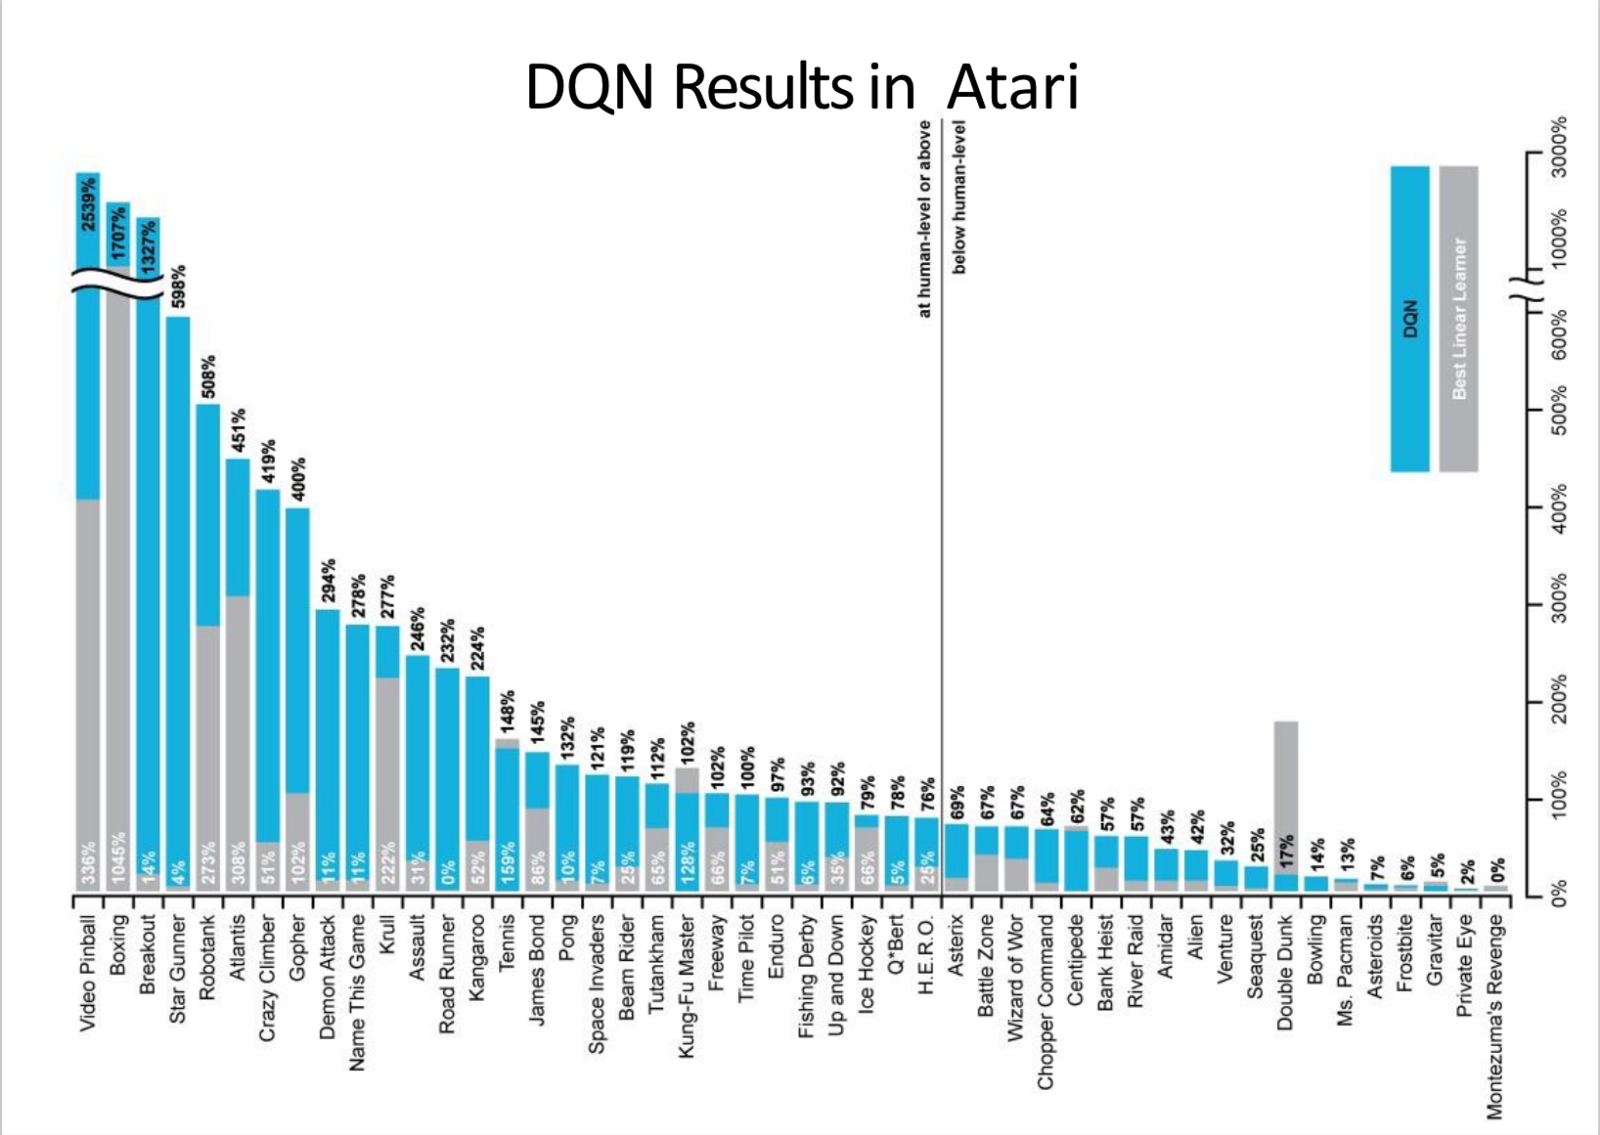
\includegraphics[height=0.35\textheight]{Chapter1/DQN-atari.png}	
	 		\caption{DQN results in Atari games}
     \end{subfigure}
     
	 \begin{subfigure}[b]{0.45\textwidth}
              \centering
	 		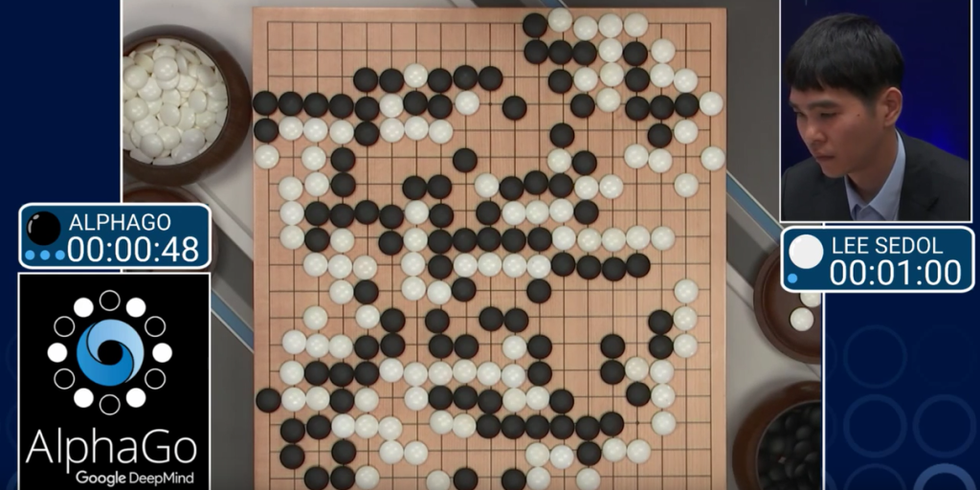
\includegraphics[height=0.2\textheight]{Chapter1/alphago.png}
	 		\caption{AlphaGo against Lee Sedol}
	 \end{subfigure}
	 ~~
      \begin{subfigure}[b]{0.45\textwidth}
              \centering
	  	    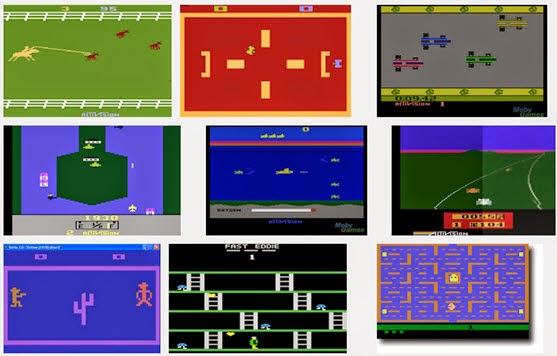
\includegraphics[height=0.2\textheight]{Chapter1/atari.jpg}
	  	    \caption{Different Atari games}
	 \end{subfigure}
	     
	 \caption{DeepMind recent achievements.}
	\label{fig:deepmind_examples}
\end{figure}

% robotics

%Another big field in Computer Science which has been receiving great attention of the research community is mobile robotics. Robotics can address state of the art challenges in different domains, such as Electronics Engineering, Mechanical Engineering, Control Theory and, of course, Machine Learning.

Another big field in Computer Science is mobile robotics, which plays a big role in the future of the industry and part of the forefront of academic research recently. Robotics can address state of the art challenges in different domains, such as Electronics Engineering, Mechanical Engineering, Control Theory and, of course, Machine Learning.

AI finds in Robotics several applications, as computer vision, path planning and even motion control, and in this last one we can find one of its biggest challenges. In Atari and board games we can easily define a goal, win, but how can we define the agility and flexibility of a walk or a jump movement? In this sense, several works have been conducted in the problem of trying to reproduce human movements in humanoid robotics agents, and more specifically, in a simulated scenario.

\begin{figure}[ht]
  	\centering
  	\begin{subfigure}[b]{0.45\textwidth}
              \centering
	 		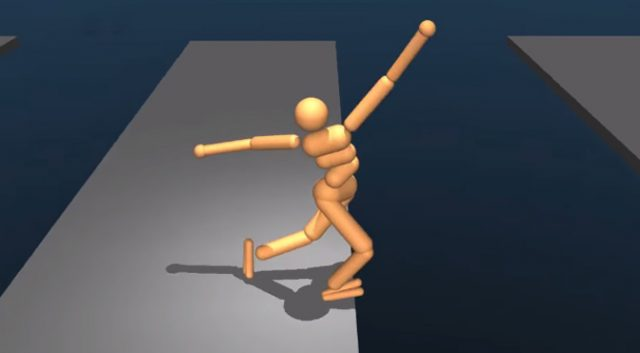
\includegraphics[height=0.13\textheight]{Chapter1/humanoid-deepmind1.jpg}	
     \end{subfigure}
     
	 \begin{subfigure}[b]{0.45\textwidth}
              \centering
	 		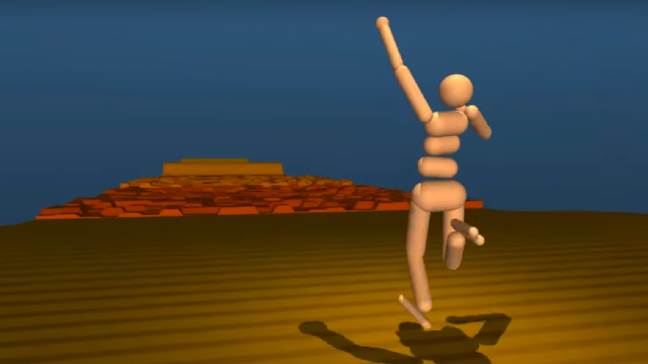
\includegraphics[height=0.13\textheight]{Chapter1/humanoid-deepmind2.png}
	 \end{subfigure}
	 ~~
      \begin{subfigure}[b]{0.45\textwidth}
              \centering
	  	    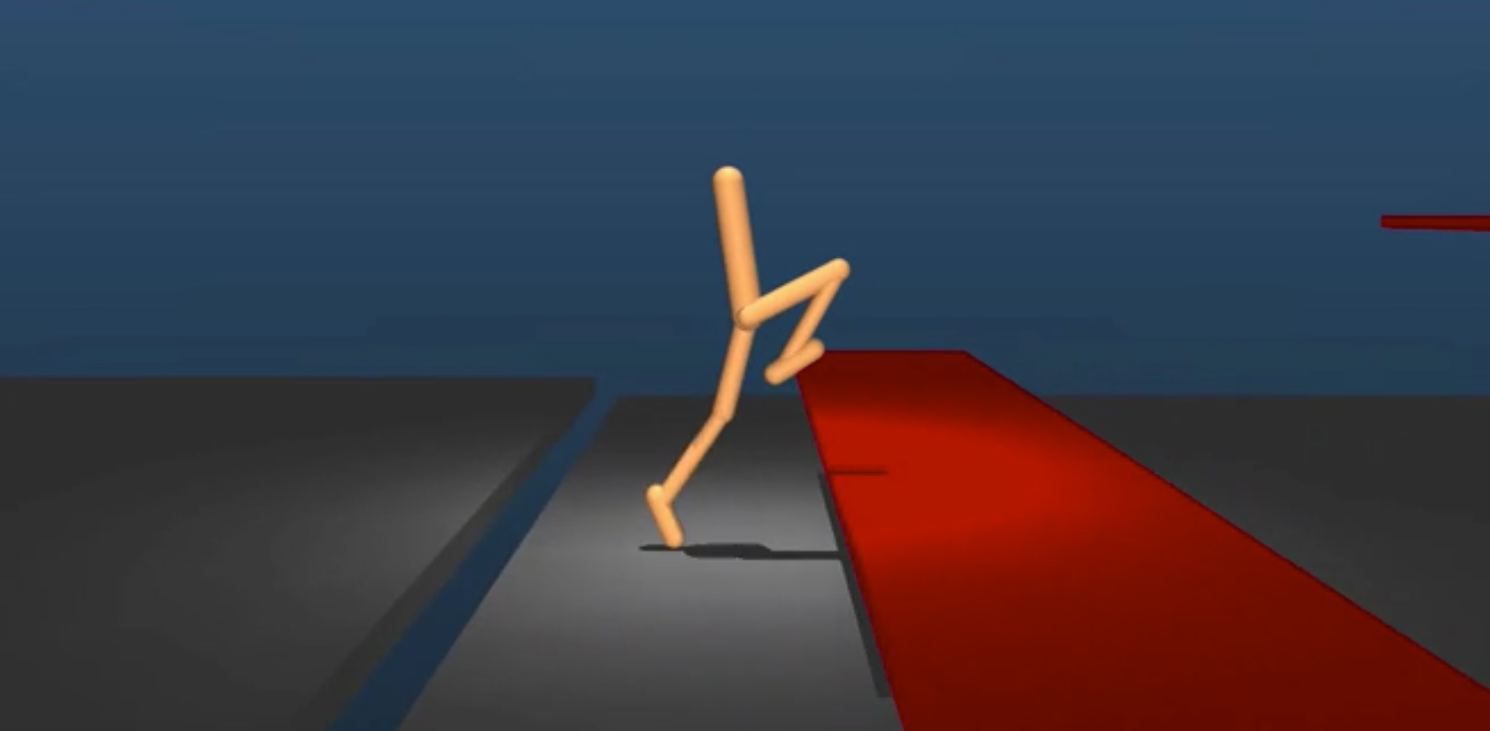
\includegraphics[height=0.13\textheight]{Chapter1/humanoid-deepmind3.png}
	 \end{subfigure}
	     
	 \caption{Simulated humanoid agent movements and AI.}
	\label{fig:humanoid_AI}
\end{figure}

% robocup

One of the biggest initiatives of the research community to foster the study of robotics is RoboCup. RoboCup established itself as one of the main international robotics competition in the world, and also organizes a scientific conference to share the latest works in the field. It pushes state-of-the-art research in robotics by maintaining different technical challenges, among them the most famous are making robots play soccer, with the mission of developing a humanoid robot team capable of win the champion of FIFA World Cup in 2050.

One RoboCup's particular league is the RoboCup 3D Soccer Simulation League, consisting of a soccer match between two teams, each one composed by up to 11 simulated NAO robots from Aldebaran Robotics. This league address both high level and low level robotics challenges, like path planning and locomotion, and greatly helped improving our understand of human movements like walk and kick the ball.

\begin{figure}[ht]
  	\centering
  	\begin{subfigure}[b]{0.45\textwidth}
              \centering
	 		
\includegraphics[height=0.13\textheight]{Chapter1/RoboCup.png}	
     \end{subfigure}
     
	 \begin{subfigure}[b]{0.45\textwidth}
              \centering
	 		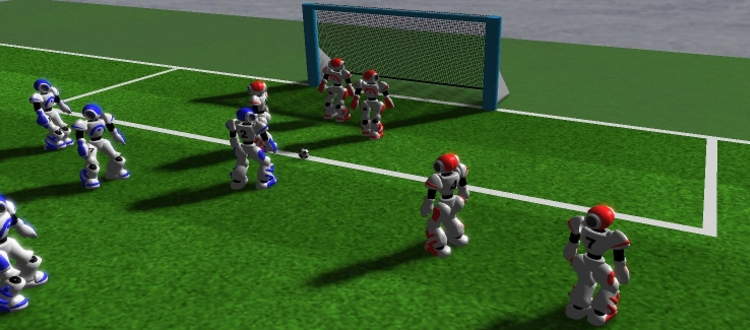
\includegraphics[height=0.13\textheight]{Chapter1/SS3D.png}
	 \end{subfigure}
	     
	 \caption{Robocup symbol and Soccer 3D Simulation league match.}
	\label{fig:robocup}
\end{figure}

\section{Problem Statement}

Inspired by the RoboCup 3D Soccer Simulation (Soccer3D or SS3D) league, this dissertation's objective is to learn a low level soccer behavior for simulated humanoid robots, more specifically, the behavior of kicking the ball towards a planned final distance from the agent. In this sense, the algorithm should input the current agent state, including its joints positions and distance to the ball, and output sequential controls for each robot's joint.

\section{Approach}

Instead of employing a deterministic and off-line built single movement, called Keyframe movement, we intend to use a model-free deep reinforcement learning based approach that tries to learn the desired behavior by interacting with an environment (the simulation server) and receiving rewards depending on which actions it chooses.
The chosen strategy for this will be first learning a behavior that imitates the current kick movement, as described in the work \cite{deepmimic}, and then improving this behavior by reinforcement learning, targeting the desired position given as an input to the policy function.
% PERGUNTAR MELHOR PRO MANGA

\section{Literature Review}

Reinforcement Learning techniques have been in increasingly study in the past 30 years. In this time, some specific works have established  famous breakthroughs in this field. For instance, Temporal-Difference (TD) learning algorithms \cite{TDLearning} created the groundwork for many future RL algorithms, making use of value function estimation and policy and value iteration methods. In the same way, Q-Learning \cite{QLearning} introduced off-policy model-free learning with \textit{Sarsa}, estimating action-value functions and making room to future DRL algorithms.

After these works, \citen{REINFORCE} created a new paradigm presenting the REINFORCE algorithm, which introduces policy search methods. This technique estimates the optimal-policy function $\pi_*$ directly, without the need of value or action-value functions and works better in continuous action space, as we see in the robotics world. The most recent approaches developed make use and improve this method, such as the Deep Deterministic Policy Gradients (DDPG) algorithm, introduced by \cite{DDPG}, the Trust Region Policy Optimization (TRPO) algorithm, presented in \cite{TRPO}, and the Proximal Policy Optimization (PPO) algorithm, given in \cite{PPO}.

Another recent breakthrough in the RL field was given by Deep Neural Networks, making possible to escalate the classical algorithms to high dimensional problems. This process was marked by the incredible results of the Deep Q-Networks (DQN) algorithm \cite{RLNature2015}. This technique was able to learn 49 Atari games directly from raw pixels of the screen. It introduces the idea of modeling the action-value function as a neural network, and handle the inherently instability problem from value function approximation by introducing also two techniques: Experience Replay \cite{ReplayBuffer} and Target Networks \cite{RLNature2015}.

Meanwhile, some recent works started to address humanoid movements in the RL field. However, the main problem which comes with that endeavor is that simple rewards functions or naively selected ones, such as the score for the games problems, can lead to results that do not match the expectations. This is the common case in continuous control tasks, like locomotion. In this sense, \cite{deepmind1} proposed that rich and robust behaviors can emerge from simple reward functions, if the environment itself contains sufficient richness and diversity. This work introduces scenarios with a lot of obstacles and varying levels of difficulty, which are presented to the agent as an implicit curriculum, making possible to overcome increasingly hard challenges. A similar idea was also introduced by \cite{BengioCurrLearning}

Other DeepMind's papers introduced methods to learn to imitate human movements, like \cite{deepmind2} and \cite{deepmind3}, which combines supervised learning and Generative Adversarial Imitation Learning (GAIL) \cite{gail}, in a way that accentuates their individual strengths and address their limitations.

Another recent state-of-the-art work in imitation learning is \cite{deepmimic}. This work makes possible for a motion capture actor to supply a set of reference motions for style, and then generate goal-directed and physically realistic behaviors from them. The approach used for this is designing a reward function which combines rewarding motions that resemble reference animation data, and also achieving additional task objectives.

The most famous work that address the specific mission of kicking the ball towards a planned final distance from the agent in the Soccer3D environment is \cite{abbas}. In this work, the authors used a policy search approach to determine the optimal parameters for the kicking behavior policy $\pi(\theta | s)$, proposing the use of contextual relative entropy policy search with covariance matrix adaptation (CREPS-CMA) algorithm for this task.

However, we can see some limitations of this work that is possible to tackle. In \cite{abbas}, the authors still make use of a Keyframe based movement, and the policy $\pi(\theta | s)$ only outputs the initial and final frame position given the desired distance $s$. We propose a neural network based policy which inputs and outputs all the joints positions in run time, performing a closed loop behavior. Besides, there are more recent and cutting-edge RL algorithms that can be used to learn this task, such as DDPG, TRPO and PPO, and also, by making use of the approach described in \cite{deepmimic}, it is possible to overcome the initial challenge of learning a basic but complete behavior at first.

At last, we must cite the work \cite{TGMuzio}, which is one of the first works covering deep reinforcement learning and the SS3D, with similar tasks regarding humanoid locomotion. More specifically, this work handles the problem of developing a behavior for dribbling the ball against a single opponent, and provide successful solutions using DDPG, TRPO and PPO.

\section{Contributions}

This work's major contribution is applying recent deep reinforcement learning (DRL) algorithms in the task of learning a complete behavior to kick a ball towards a planned final distance from the agent in the Soccer3D environment domain. To the best of our knowledge, this work is the first that makes use of a DRL approach to develop a complete soccer behavior for this specific task.

\section{Outline of this Dissertation}

This dissertation is organized as follows:

\begin{itemize}
    \item \textbf{Chapter \ref{chap:introduction}} introduces this dissertation by describing the motivation 
    behind the problem we address, by the Literature review and by summarizing the contributions.

    \item \textbf{Chapter \ref{chap:rl}} describes a brief theoretical background of reinforcement learning and neural networks.
    
    \item \textbf{Chapter \ref{chap:deep_rl}} describes a brief theoretical background of neural networks and some cutting-edge DRL algorithms

%    \item \textbf{Chapter \ref{chap:deep_learning}} constructs the building blocks of deep learning.

%    \item \textbf{Chapter \ref{chap:deep_rl}} provides the main deep reinforcement learning techniques used in our work.

%    \item \textbf{Chapter \ref{chap:methodology}} explains the methodology of this work, the tools that were used and how 
%    our environment was implemented.

%    \item \textbf{Chapter \ref{chap:contrib}} describes this dissertation's major contributions: 
%    how we formulated the learning tasks and how we modeled it to successfully
%    master them.

%    \item \textbf{Chapter \ref{chap:experiments}} evaluates our model in a few humanoid soccer tasks and describes our results.

%    \item \textbf{Chapter \ref{chap:conclusion}} concludes this dissertation and presents our ideas for future investigation.
\end{itemize}


\chapter{Reinforcement Learning}
\label{chap:rl}
\section{Model Introduction}

Reinforcement Learning is a new branch and paradigm in the Machine Learning field. But different than the classical Supervised Learning, in RL there is no supervisor, only a reward signal. In this sense, we have an agent which interacts with the environment and receives instant rewards. Therefore, in RL, we can say that the agent's actions affect the subsequent data it receives, and that time really matters, since this data is sequential non i.i.d, and moreover, the total feedback, given by the sum of all rewards, is delayed, not instantaneous \cite{Sutton1998}. All these features make RL a quite unique research field, and it can also finds a wide range of applications, from playing board games to machines control.

The basic model for a RL approach makes use of a discrete state space for representing the agent's state $S_t$, its actions $A_t$ and its full or partial environment observations $O_t$. Thus, at each timestep $t$, the agent receives an observation $O_t$, takes an action $A_t$ and ends up in the next state $S_{t+1}$, receiving an scalar reward $R_{t+1}$. Therefore, the agent's final goal is to maximize the total future reward it gets. Figure \ref{fig:RL_basic_model} illustrates this dynamics representation.

\begin{figure}[H]
    \centering
    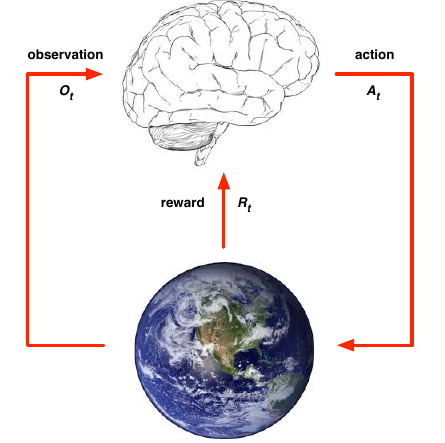
\includegraphics[width=0.4\textwidth]{Chapter2/RL_basic_model.png} 
    \caption{Agent interacting with environment.}
    \label{fig:RL_basic_model}
\end{figure}


\section{Markov Decision Processes}

A classic formal description of an environment for reinforcement learning makes use of Markov decision processes, which inherits the Markov Property from the well known first-order Markov chains. In these Markov chains, we establish that the state of the agent captures all the relevant information from the history, in other words, the probability update function only depends of the immediate previous state, as described in Equation \eqref{eq:markov_basic}.

\begin{equation}
P(S_{t+1} | S_t) = P(S_{t+1} \mid S_1, ..., S_t)
\label{eq:markov_basic}
\end{equation}

Markov decision processes, however, have a more complete definition, they are a Markov process with rewards and actions. Basically, can be represented as a tuple $<\textbf{S}, \textbf{A}, P, R, \gamma>$, with each component defined as follows:
\begin{itemize}
\item
	$\textbf{S}$ is a finite set of states the agent can assume in the environment.
\item
	$\textbf{A}$ is a finite set of actions the agent can take.
\item
	$P$ is a state transition probability function, represented as $P_{ss'}^a = \mathbb{P}[S_{t+1}=s' \mid S_t = s, A_t = a]$
\item
	$R$ is the immediate reward function, with expected value given by $R_s^a = \mathbb{E}[R_{t+1} \mid S_t = s, A_t = a]$
\item
	$\gamma$ is a discount factor, such that $\gamma \in [0,1]$, used to compute the cumulative total reward.
	
\end{itemize}

Besides this basic tuple representation, there are four more concepts very used in the RL literature that we must present.

\begin{itemize}
\item
	The \textbf{return} $G_T$ is the total discounted reward from time-step t, given by:
	\begin{equation}
	G_t = R_{t+1} + \gamma R_{t+2} + ... = \sum_{k=0}^{\infty}{\gamma^k R_{t+k+1}}
	\end{equation}
	Notice that by introducing the discount factor $\gamma$, it is possible to set the agent preference between short-term and long-term rewards.
\item
	The \textbf{policy} $\pi(a \mid s)$ is a probability distribution function over actions given states, defined by:
	\begin{equation}
	\pi(a \mid s) = \mathbb{P}[A_t=a | S_t=s]
	\end{equation}
	The policy fully defines the behavior of the an agent, and can also be deterministic.
\item
	The \textbf{state-value function} $v_{\pi}(s)$ is the expected return starting from state $s$ and then following a policy $\pi$.
	\begin{equation}
	v_{\pi}(s) = \mathbb{E}_{\pi}[G_t \mid S_t = s]
	\label{eq:state_value_function_definition}
	\end{equation}
	In other words, it can be seen as a measure of how good the current agent's state is.
\item
	The \textbf{action-value function} $q_{\pi}(s,a)$ is the expected return starting from state $s$, taking action $a$, and then following policy $\pi$
	\begin{equation}
	q_{\pi}(s,a) = \mathbb{E}_{\pi}(G_t \mid S_t = s, A_t = a)
	\label{eq:action_value_function_definition}
	\end{equation}
	It can also be understood as a measure of how good it is to take a given action at the agent's current state.
\end{itemize}

\subsection{Optimality in Reinforcement Learning}

The ultimate goal of RL is finding an optimal behavior that maximizes the total expected return given by $\mathbb{E}_{R_i,S_i \sim E, A_i \sim \pi}[G_i]$. Before starting presenting the methods for achieving this goal, we must define what is optimality for value functions and policies.

\subsubsection{Optimal Value Function}

A value function is optimal if it is the maximum over all policies for all states (or state-action pairs).
\begin{itemize}
\item
	Optimal State-value function: $v_*(s) = \underset{\pi}{\textrm{max }} v_\pi(s)$
\item
	Optimal Action-value function: $q_*(s, a) = \underset{\pi}{\textrm{max }} q_\pi(s, a)$.
\end{itemize}

The optimal value functions specify the best possible performance in the MDP, which is only ``solved'' when we know the optimal value functions.

\subsubsection{Optimal Policy}

First, we must define a partial ordering over policies, given in Equation \eqref{eq:policy_ordering}.

\begin{equation}
\pi \geq \pi' \text{ if } v_{\pi}(s) \geq v_{\pi'}(s), \forall s
\label{eq:policy_ordering}
\end{equation}

The optimal policy $\pi_*$ is then defined as the best among all the others policies $\pi$, such that $\pi_* \geq \pi, \forall \pi$. Moreover, the following theorem introduces three fundamental properties about optimal policies.

\begin{itemize}
\item
There exists an optimal policy $\pi_*$ that is better than or equal to all other policies, $\pi_* \geq \pi, \forall \pi$.
\item
All optimal policies achieve the optimal value function, $v_{\pi_*}(s) = v_*(s)$.
\item
All optimal policies achieve the optimal action-value function, $q_{\pi_*}(s,a) = q_*(s,a)$.
\end{itemize}

Furthermore, a deterministic optimal policy always exists, and can be easily defined from the optimal action-value function, as described in Equation \eqref{eq:policy_from_greedy}.

\begin{equation}
 \pi_*(a | s) = 
\begin{cases}
    1,& \text{if } a = \underset{a'}{\textrm{argmax }} q_*(s,a')\\
    0,& \text{otherwise}
\end{cases}
\label{eq:policy_from_greedy}
\end{equation}

\section{RL Algorithms}

In order to base our future approaches in the main task, we must start presenting the classical reinforcement learning algorithms in the literature and, first of all, categorizing its different natures. The following subsections will be responsible for that.

\subsection{Categorizing RL}

RL algorithms can be classified into several types related to their problems and solutions approaches.

%RL algorithms can be classified into model free or model based, prediction or control, and value based, policy based or actor critic.

Model based algorithms are used when the model of the environment is known, and therefore, the agent can performs computations without external interaction to improves its policy. Model free algorithms, however, do not use any environment model, and it improves its policy by only interacting with the environment. These two problems conditions are respectively classified as planning and reinforcement learning problems.

Moreover, RL algorithms can also be classified as value based, policy based or actor critic. Value based algorithms are methods based on computing optimal value functions, whereas policy based algorithms make use of optimal policy search approaches. Between them, we also have an hybrid solution which combines both value function and policy search approaches. Figure \ref{fig:categorizing_RL}, extracted from \cite{lecture1DS}, illustrates this classical RL categories division.

Regarding their solution nature, we also have two more classifications. Prediction algorithms are basically policy evaluation algorithms, which does not obtain any optimal policy solution, but instead, given a policy computes value functions. Control algorithms, whereas, aims to achieve an optimal policy. Besides, we still have two other classifications regarding the solution approach, that are on-policy algorithms, which learns by interacting with the world with its own policy, and off-policy algorithms, which learns an optimal policy by interacting with the world with another policy.

%Explica on e off-policy


\begin{figure}[H]
    \centering
    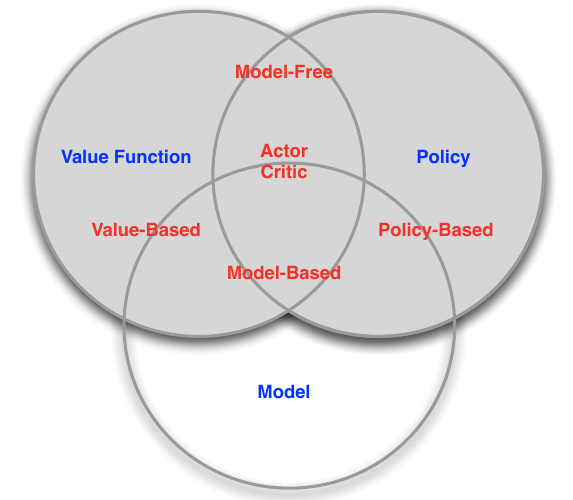
\includegraphics[width=0.5\textwidth]{Chapter2/categorizing_RL.png} 
    \caption{Classical division among RL algorithms classifications.}
    \label{fig:categorizing_RL}
\end{figure}

\subsection{Value Function Methods}

As already mentioned, value function methods employ techniques that aims to compute or estimate value functions. These algorithms are the most classic in the RL literature, and their implementation differ basically in relation to concepts like bootstrapping, bias, variance, on-policy and off-policy. In this section, we will focus on presenting only model-free algorithms, since it is from the same nature of our problem.

\subsubsection{Monte Carlo Methods}

Monte Carlo or MC methods \cite{Sutton1998} are model-free methods that learn directly from full episodes of experience. It computes value functions through its expectation definition given in Equations \eqref{eq:state_value_function_definition} and \eqref{eq:action_value_function_definition}. However, without a known model for the MDP, it estimates this expectation by sampling and computing the empirical mean return.

Therefore, for Monte Carlo prediction, the MC version for policy evaluation, we compute the state value $v_{\pi}(s)$ by averaging full episodic returns starting from state $s$ and running on policy $\pi$ for an arbitrarily large number of episodes in this condition.

For the control method, the main idea is to employ policy iteration, which is a basic framework for control problems which consists in an iterative solution that evaluates a given policy, by computing the value functions, and then updates this policy by acting greedy with respect to these computed value functions. Acting greedy would be choosing a deterministic policy given by Equation \eqref{eq:policy_from_greedy}. This loop repeats until convergence to optimal policy and optimal value functions.

In Monte Carlo model-free control, in particular, the usual approach is to use Monte-Carlo prediction to evaluate action-value functions $Q_{\pi}(s,a)$ under the policy $\pi$, then update the policy acting $\epsilon$-greedy. $\epsilon$-greedy is a simple policy update technique very similar to the greedy approach from \eqref{eq:policy_from_greedy}, but it is able to ensure continual exploration. The solution for this is choosing the greedy action with $1-\epsilon$ probability, and all the others actions with the same non-zero probability. This calculation is presented in Equation \eqref{eq:epsilon-greedy}.

\begin{equation}
 \pi_*(a | s) = 
 \begin{cases}
    \epsilon/m + 1 - \epsilon ,& \text{if } a = \underset{a'}{\textrm{argmax }} q_*(s,a')\\
    \epsilon/m ,& \text{otherwise}
 \end{cases}
 \label{eq:epsilon-greedy}
\end{equation}

%It is possible by making that the greedy action be chosen with $1-\epsilon$ probability, whereas 

% Monte Carlo Prediction slides 6 e 7 lecture 4
% Monte Carlo Control    slides 13 ao 16 lecture 5
% Explica epsilon-greedy

\subsubsection{Temporal-Difference and Sarsa}

Temporal-Difference methods \cite{Sutton1998} and \cite{TDLearning} are model-free methods that are able to learn from incomplete episodes, by bootstrapping. This idea consists in updating an estimate by using another estimate obtained after taking some decision steps. In its most simple version for policy evaluation, $TD(0)$, it is possible to learn $v_{\pi}$ online while experiencing under $\pi$, by updating the estimate $V(S_t)$ toward the estimated return $R_{t+1} + \gamma V(S_{t+1})$, as given in Equation \eqref{eq:TD0_update}.

\begin{equation}
V(S_t) = V(S_t) + \alpha(R_{t+1} + \gamma V(S_{t+1}) - V(S_t))
\label{eq:TD0_update}
\end{equation}

For Temporal-Difference control, it is also commonly employed a policy iteration approach. We use TD to compute action-value function estimates $Q(S,A)$ given the policy $\pi$, and then use $\epsilon$-greedy to improve the policy. This method is known as SARSA, due to the process of, given a state $S$, take an action $A$, receive a reward $R$, end in a next state $S'$, and then choose another action $A'$ in order to compute the TD target. The Algorithm \ref{algo:sarsa} fully describes this method.

\begin{algorithm}[H]
    \DontPrintSemicolon
    \SetAlgoLined
    Initialize $Q(s,a)$, $\forall s \in S$, $a \in A(s)$, arbitrarily, and $Q$(terminal-state,.)=0\;
    \For{episode = $1$, $M$}{
        Initiliaze $S$\;
        Choose $A$ from $S$ using policy derived from $Q$ (e.g., $\epsilon$-greedy). \;
        \For{t = $1$, ...,$T$}{
			Take action $A$, observe $R$, $S'$. \;
			Choose $A'$ from $S'$ using policy derived from $Q$ (e.g., $\epsilon$-greedy). \;
			$Q(S,A) \leftarrow Q(S,A) + \alpha(R + \gamma Q(S',A') - Q(S,A))$. \;
			$S \leftarrow S'$; $A \leftarrow A'$; \;
        }
    }
    \caption{Sarsa algorithm}
    \label{algo:sarsa}
\end{algorithm}

The SARSA algorithm is more famous for another variation, that is able to bootstrap into more future steps. The SARSA($\lambda$) method computes a different TD target $Q_t^{\lambda}$ making use of a discount weight $(1-\lambda) \lambda^{n-1}$ over $n$ steps action-values $Q_t^{(n)}$, as shown in Equation \eqref{eq:sarsa_lambda}.

\begin{align}
Q_t^{\lambda} = (1 - \lambda) \sum_{i=1}^{n}{\lambda^{n-1}Q_t^{(n)}} \\
Q(S,A) = Q(S,A) + \alpha( Q_t^{\lambda} - Q(S,A))
\label{eq:sarsa_lambda}
\end{align}

The main difference between SARSA and MC control algorithms is that SARSA can learns before the end of the episode, and have low variance and some bias, whereas MC can only learn from complete episodes, and therefore has high variance and zero bias. Besides, MC has better convergence properties.

% TD lambda para prediction
% TD lambda para control com Sarsa slides 23 ao 25 lecture 5, apresentar algoritmo

\subsubsection{Q-Learning}

For off-policy learning we have some variations of the previous algorithms. The most basic ones, like Off-Policy MC and Off-Policy TD \cite{Sutton1998}, involve importance sampling, that corrects expectations given in one distribution to another, as shown in Equation \eqref{eq:importance_sampling}.

\begin{equation}
\mathbb{E}_{X \sim P}[f(X)] = \mathbb{E}_{X \sim Q}\left[\frac{P(X)}{Q(X)}f(X)\right]
\label{eq:importance_sampling}
\end{equation}

The most famous off-policy algorithm though is Q-learning \cite{QLearning}, that does not importance sample. Q-learning is able to improve both the behavior policy $\mu$ and the target policy $\pi$, by acting greedy w.r.t. $Q(s,a)$ for $\pi$ and acting $\epsilon$-greedy w.r.t. $Q(s,a)$ for $\mu$. The general algorithm is very similar to SARSA, with the difference that the next action is chosen using the behavior policy, and the alternative successor action is chosen using the target policy. Equation \eqref{eq:qlearning_update} describes the update step for $Q(S,A)$ in Q-learning.

\begin{equation}
Q(S,A) \leftarrow Q(S,A) + \alpha (R + \gamma \underset{a'}{\textrm{max }}Q(S',a') - Q(S,A))
\label{eq:qlearning_update}
\end{equation}

\subsection{Policy Search Methods}

Policy search methods are model-free control algorithms which directly compute the optimal value function without the use of value functions estimates, as shown in previous algorithms. In this sense, the approach consists in using a parametrized function approximation $\pi_{\theta}(a|s)$ for the policy, and the goal is to reach the desired parameters $\theta^*$ that best estimate the optimal policy, in a way that $\pi_{\theta^*}(a|s) \thickapprox \pi_*(a|s)$. Furthermore, the strategy for achieving this goal is solving an optimization problem, which comes from another perspective for the optimal policy, that is the policy that maximizes the expected total return running over several trajectories $\tau$, as defined in Equations \eqref{eq:tau_def} and \eqref{eq:theta_max}.

\begin{align}
P_{\theta}(\tau) = P_{\theta}(s_1,a_1,...,s_T,a_T) = P(s_1)\prod_{t=1}^T{\pi_{\theta}(a_t|s_t) P(s_{t+1}|s_t,a_t)} 
\label{eq:tau_def}
\\
\theta^* = \underset{\theta}{\textrm{argmax }} J(\theta) =
\underset{\theta}{\textrm{argmax }} \mathbb{E}_{\tau \sim P_{\theta}(\tau)} \left[ \sum_t{R_t(s_t,a_t)} \right]
\label{eq:theta_max}
\end{align}

This optimization problem is solved through gradient ascent methods, and therefore we must compute the gradient of the objective function $J(\theta)$. For this propose, we can rewrite $J(\theta)$ as in \ref{eq:rewrite_objective}, and compute its gradient $\nabla_{\theta} J(\theta)$ using the manipulation described in \ref{eq:grad_with_scorefunc}, in order to work with the score function $\nabla_{\theta}\log{\pi_{\theta}(a|s)}$.

\begin{equation}
J(\theta) = \mathbb{E}_{\tau \sim P_{\theta}(\tau)} \underbrace{ \left[ \sum_t{R_t(s_t,a_t)} \right] }_{r(\tau)} = \int{\pi_{\theta}(\tau)r(\tau)d \tau}
\label{eq:rewrite_objective}
\end{equation}

\begin{equation}
\nabla_{\theta} J(\theta) = \int{\nabla_{\theta} \pi_{\theta}(\tau)r(\tau)d \tau} = 
\int{\pi_{\theta}(\tau) \nabla_{\theta} \log{\pi_{\theta}(\tau)} r(\tau)d \tau} =
\mathbb{E}_{\tau \sim \pi_{\theta}(\tau)} \left[ \nabla_{\theta} \log{\pi_{\theta}(\tau)} r(\tau) \right]
\label{eq:grad_with_scorefunc}
\end{equation}

Using the gradient $\nabla_{\theta} J(\theta)$, computed in \ref{eq:grad_with_scorefunc}, the main idea presented in \cite{REINFORCE} is making use of stochastic gradient ascent to reach $\theta^*$. The algorithm is therefore presented in Algorithm \ref{algo:reinforce}.

\begin{algorithm}[H]
    \DontPrintSemicolon
    \SetAlgoLined
    Initialize $\theta$ arbitrarily\;
    \For{each episode \{ $s_1$, $a_1$, $r_2$, ..., $s_{T-1}$, $a_{T-1}$, $r_T$ \} $\sim$ $\pi_{\theta}$ }{
        \For{t = $1$, ...,$T$}{
			$\theta \leftarrow \theta + \alpha \nabla_{\theta} \log{\pi_{\theta}(s_t,a_t)} G_t$
        }
    }
    \Return{$\theta$}
    \caption{REINFORCE algorithm}
    \label{algo:reinforce}
\end{algorithm}

In comparison with value function methods, the main advantages of policy-based RL algorithms are the effectiveness in high-dimensional or continuous action spaces, the possibility to learn stochastic policies and the better convergence properties. The main disadvantages, though, are the computational inefficiency, the high variance of these methods and the usual convergence to local optimum rather than the global optimum.

% define average reward objective function
% define the goal for RL, that is theta argmax J(theta)
% derive grad J(theta) with score function and sum total reward
% present REINFORCE algo

\subsection{Actor-Critic}
% presenting the critic Qw(s,a) as a function estimate for the total return Gt

In Algorithm \ref{algo:reinforce}, we used the total return $G_t$ as an unbiased sample of $Q^{\pi_{\theta}}(s_t,a_t)$, but we can also rewrite $\nabla_{\theta} J(\theta)$ as in equation \ref{eq:actor_critic_gradient}. In this sense, we could also use an action-value function approximation to derive the objective function gradient, by making use of a \textit{critic} function $Q_W(s,a) \thickapprox Q^{\pi_{\theta}}(s_t,a_t)$.

\begin{equation}
\nabla_{\theta} J(\theta) = \mathbb{E}_{\tau \sim \pi_{\theta}(\tau)} \left[ \nabla_{\theta} \log{\pi_{\theta}(\tau)} Q^{\pi_{\theta}}(s_t,a_t) \right]
\label{eq:actor_critic_gradient}
\end{equation}

Therefore, Actor-Critic methods maintain two sets of parameters to be updated toward optimum policy and action-value functions: the parameters $W$ for the \textit{critic} action-value estimate $Q_W(s,a)$, and the parameters $\theta$ for the \textit{actor} policy estimate $\pi_{\theta^*}(a|s)$.



%\chapter{Deep Learning}
%\label{chap:deep_learning}
%In the last chapter we described the mathematical background behind reinforcement learning and how a problem can be modeled with it.
We also saw that for problems with continuous state and/or action spaces, it can be necessary to use function approximators such as
neural networks. 
In this chapter we  will describe the theoretical background of NNs, as function approximators.

Deep learning is a field of Machine Learning that in part studies deep neural networks and how they learn. 

\section{History}
Today, Deep learning is a very significant topic for the scientific community yet its history goes back since the 1940s \cite{DeepLearningBook}.

There has been a major resurgence of deep learning mainly because computers today became faster.
Training large deep learning models are computationally very expensive and could be sped up with the use
of graphics processing units (GPUs).

Artificial Neural Networks are one of the earliest learning algorithms. The novel concept behind it was to 
create mathematical models that tried to mimic the brain.
NNs were based on the human brain's neurological structure, more specifically neurons and how they connect with other neurons.
Figure \ref{fig:neuron} illustrates a single neuron cell.

\begin{figure}
    \centering
    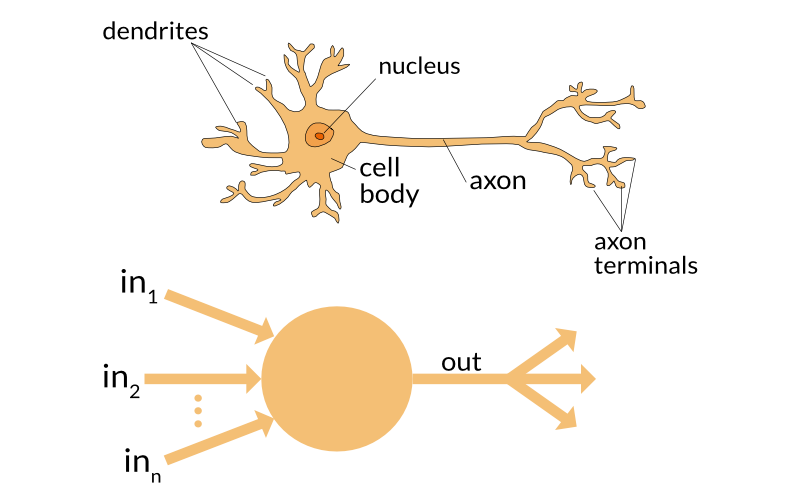
\includegraphics[width=1\textwidth]{Chapter3/neuron.png}
    \caption{Neuron unit cell structure.}
    \label{fig:neuron}
\end{figure}

A neuron cell is capable of transmitting information by sending electrical and chemical signals through axons and they connect to other neurons
forming neural networks. The human brain, for example, has billions of connected neurons.
NNs, therefore, are a simplified mathematical representation of neurons: essentially, a neuron can be viewed as a cell that receives one or more inputs
and produces one or more outputs.

\section{Neural Networks}

\subsection{Representation}
\label{sec:rep}

In simple terms, a neural network is a mathematical structure that receives an input and calculates an output.
We will describe a simple NN known as feedforward neural network or Multi Layer Perceptron (MLP).

A neural network is composed of multiple layers where each layer has one or more nodes (neurons).
The NN receives an input and computes the output according to the network architecture and parameters $\theta$.
Each input, called sample or example, is a n-dimensional feature vector $x$, and is represented as a column vector:

\begin{equation}
    x = \begin{bmatrix}
            x_1 & x_2 & x_3 & x_4 & \dots & x_{n-1} & x_{n}
        \end{bmatrix}^\intercal
\end{equation}

$x$ is known as the input layer, and each coordinate represents each of the sample's features.
The output is a k-dimensional vector $y$, known as the output layer. 
Every other layer that is not the input nor the output layer is known as a hidden layer.

In this work, note that every time we refer to an element $z^{[l]}$ we are referring to an element of the $l$-th layer.

Figure \ref{fig:neuralnet} illustrates a very simple NN with a 3-dimensional feature vector, 1-dimensional output vector and only one hidden layer.

\begin{figure}[ht]
    \centering
    \includegraphics[width=0.75\textwidth]{Chapter3/neuralnet.pdf}
    \caption{Simple neural network.}
    \label{fig:neuralnet}
\end{figure}

Every node of the network is computed using the values from the previous layer. 
For the MLP, the node computation model is done through
a linear model $f(x; \theta)$, with $\theta$ consisting of internal parameters $w$ (weights) and $b$ (bias).
$w$ has the same dimensions as the input and $b$ is a scalar.
In this work, we treat $w$ as a column vector.

\begin{equation}
    w = \begin{bmatrix}
            w_1 & w_2 & w_3 & w_4 & \dots & w_{n-1} & w_{n}
        \end{bmatrix}^\intercal
\end{equation}

The model is defined as

\begin{equation}
    z = w^Tx + b
\end{equation}

The output of the node $a$, also known as the activation, is calculated with $x$, $b$ and 
a function $\sigma : \mathbb{R} \rightarrow \mathbb{R}$:

\begin{equation}
    a = \sigma(z) = \sigma(w^T x + b) = \sigma \bigg(\sum_{i=1}^n w_i x_i + b \bigg)
\end{equation}

Figure \ref{fig:neuralnet_out} illustrates the output of a single neuron.

\begin{figure}[ht]
    \centering
    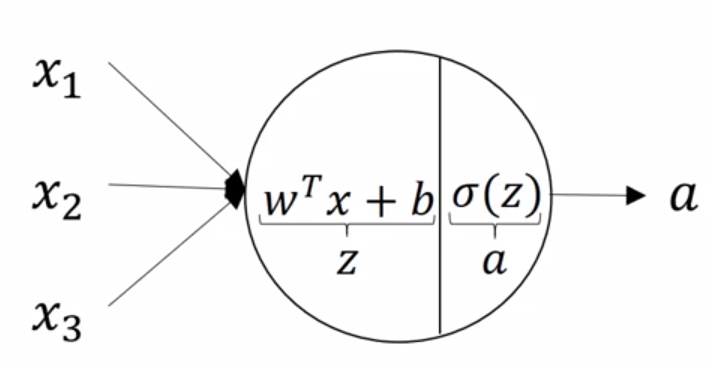
\includegraphics[width=0.6\textwidth]{Chapter3/neuralnet_output.png}
    \caption{Node computation.}
    \label{fig:neuralnet_out}
\end{figure}

$\sigma$ is called activation function, applied to the model output ($z$).
The activation function normally is a non-linear function and its most used common choice
today is the \textbf{rectified linear unit} \cite{ReLU} or ReLU
and is defined as $\sigma(z) = max\{z, 0\}$, shown in \ref{fig:relu}. 

\begin{figure}[h]
    \centering
    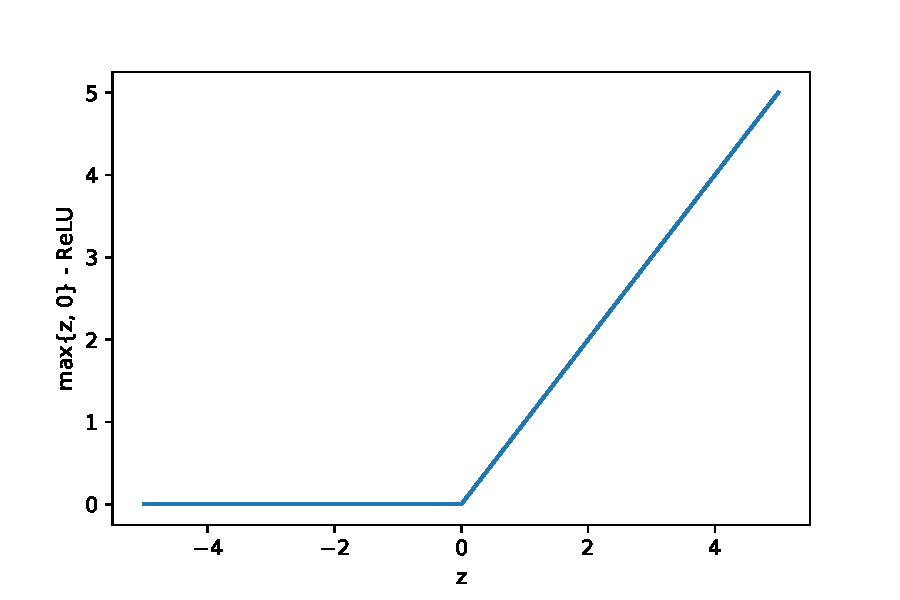
\includegraphics[width=0.75\textwidth]{Chapter3/relu.pdf}
    \caption{Linear rectified unit plot.}
    \label{fig:relu}
\end{figure}

Other examples of popular activation functions are $\sigma(z) = \frac{1}{1 + e^{-z}}$, known as the sigmoid function
and $tanh(z)$ \cite{ActivationFunction}.

A neural network is therefore is a connection of multiple neurons as inputs to other neurons.
Let us return our attention to the network from Figure \ref{fig:neuralnet}.
We denote $(W,b) = (W^{[1]}, b^{[1]}, W^{[2]}, b^{[2]})$ as the network parameters, where $W^{[l]}$ is 
the matrix formed by concatenating the individual parameters of the $l$-th layer such that
$W_{ij}$ denotes the parameter associated with the connection between neuron $j$ from the $l$-th layer 
and neuron $i$ from layer $l + 1$.
Similarly, $b^{[l]}$ is the concatenation of the biases $b$ of each neuron of layer $l + 1$ and 
$b_i^{[l]}$ the bias of the $i$-th neuron of layer $l + 1$.

For the network depicted in Figure \ref{fig:neuralnet}, we are now capable of calculating the output $y$.

For the first layer: 

\begin{equation}
    z^{[1]}  = W^{[1]}x + b^{[1]} 
\end{equation}

\begin{equation}
   a^{[1]}  = \sigma(z^{[1]})
\end{equation}

And for the second layer:

\begin{equation}
    z^{[2]} = W^{[2]}a^{[1]} + b^{[2]}
\end{equation}

\begin{equation}
    y = a^{[2]} = \sigma(z^{[2]})
\end{equation}

We can think of the neural network as a recursive structure where each activation is calculated with the past's layers activation.
$a^{[l]}$ can be computed as:

\begin{equation}
    z^{[l]} = W^{[l]}a^{[l-1]} + b^{[l]}
    \label{eq:nn}
\end{equation}

\begin{equation}
    a^{[l]} = \sigma(z^{[l]})
\end{equation}

Note also that $a^{[1]} = x$.

\subsection{Vectorization}

In the previous section, we focused on computing the output of the neural network given a single sample $x$.
In modern days, however,  we are normally interested in calculating the output of a neural network for thousands or even millions of samples.

For $m$ samples, we could naively compute the output of the neural network for each example $x^{(i)}$ with Algorithm \ref{algo:naive_sample_algo}.

\begin{algorithm}[H]
    \DontPrintSemicolon
    \SetAlgoLined
    \KwResult{Output of NN for m samples.}
    \For{i = 1 to m}{
       $a^{[0]} = x^{(i)}$\;
        \For{j = 1 to L}{
            $z^{[j](i)} = W^{[j]}a^{[j-1](i)} + b^{[j]}$\;
            $a^{[j](i)} = \sigma(z^{[j](i)})$\;
        }
        $y^{(i)} = a^{[l](i)}$\;
    }
    \caption{Naive algorithm for computing NN output of $m$ samples.}
    \label{algo:naive_sample_algo}
\end{algorithm}

In practice this algorithm runs relatively slow since it computes the output of the network sequentially for each sample and 
we will apply vectorization to achieve a much faster algorithm.

Firstly, Vectorization is a technique that transforms a set of computations done sequentially in a for loop into matrix operations.
We will now vectorize our initial problem.

Let us define the following matrices

\begin{itemize}
    \item $X$ is a matrix where column i is the i-th sample $x^{(i)}$ and $W^{[l]}$. 
    We can analogously define matrices A and Z.
        $ X = \begin{bmatrix}
        x^{(1)} & x^{(2)} &  \dots  & x^{(m)} 
        \end{bmatrix}$.

    \item $W^{[l]}$ is the  weight matrix for the $l$-layer, as defined in Section \ref{sec:rep}. 
        % $ W^{[l]} = \begin{bmatrix}
        % \left(w^{[1]})\right)^T \\ \left(w^{[2]})\right)^T \\  \vdots  \\\left(w^{[l]})\right)^T} 
        % \end{bmatrix}$.
    \item $b^{[l]}$ is the bias vector for layer $l$, as defined in Section \ref{sec:rep}.
        % $ B^{[l]} = \begin{bmatrix}
        % b^{[1]} \\ b^{[2]} \\  \vdots \\ b^{[l]}
        % \end{bmatrix}$.
\end{itemize}

For the vectorized version of Algorithm \ref{algo:vectorized_sample}.

\begin{algorithm}[H]
    \DontPrintSemicolon
    \SetAlgoLined
    \KwResult{Output of NN for m samples.}
    \For{j = 1 to L}{
        $Z^{[j]} = W^{[j]}A^{[j-1]} + b^{[j]}$\;
        $A^{[j]} = \sigma(Z^{[j]})$\;
    }
    \caption{Vectorized algorithm for computing NN output of $m$ samples.}
    \label{algo:vectorized_sample}
\end{algorithm}

The vectorized version is much better since these matrices operations can be greatly sped up
on GPUs or hardware that have support for Streaming SIMD Extensions (SSE). The great majority of 
popular deep learning libraries use as much vectorization as they can.

\subsection{Deep Neural Networks}

We can extend the architecture we saw on Section \ref{sec:rep} to a higher number of layers called
deep neural networks. Figure \ref{fig:deepnn} illustrates a neural network with multiple hidden layers.

\begin{figure}[h]
    \centering
    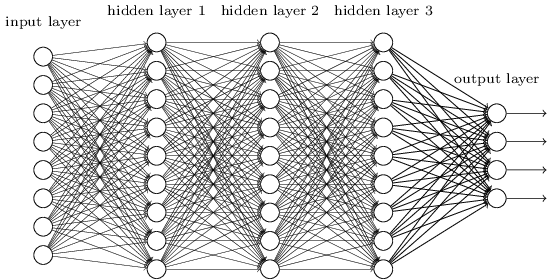
\includegraphics[width=1\textwidth]{Chapter3/deep_neural_net.png}
    \caption{Neural network with multiple layer.}
    \label{fig:deepnn}
\end{figure}

The activation of layer $l + 1, l > 1$, can be calculated according to Equation \ref{eq:nn}.

\section{Learning}

As described in the previous section, feedforward networks defines a mapping $y = f(x; \theta)$,
or, equivalently, serve as general function approximators.

This section describes deep learning algorithms that learn the value of the parameters $\theta$ that best approximates $f$.

Most deep learning algorithms need to describe a cost function and optimization algorithm.

\subsection{Cost Function}

The cost function $J(\theta)$ is a metric of how good our estimator is to our dataset: the lower the cost function, the less error
the model has when predicting $y$. It describes the function that we wish to minimize and normally it envolves an average of the errors
between the the target value of a sample and the predicted value of the estimator for the sample.

For example, for the problem of linear regression where $X$ are the sample values and $y$ are the target
values for our dataset, we wish to learn the parameters $\theta$ from our function approximator $f$. 
The most used cost function for this problem is

\begin{equation}
    J(\theta) = \dfrac{1}{m} \sum_{i = 1}^m (y_i - f(x_i, \theta))^2
\end{equation}

Another example is the logistic regression problem. The most common cost function for this problem is

\begin{equation}
    J(\theta) = - \dfrac{1}{m} \sum_{i = 1}^m [y_i\log{f(x_i, \theta} + (1 - y_i)\log{1 - f(x_i, \theta)}]
\end{equation}

Choosing a good cost function greatly impacts how good the design of the deep neural network is.

% TODO Regularization

\subsection{Optimization Algorithms}

After defining a cost function, finding the parameters that effectively minimize the cost function is not trivial.
The non linearity of NN causes most cost functions to be non-convex and therefore, neural networks are usually
trained by iterative, gradient-based optimizers. In practice, however, this is very unlikely
 \cite{swirszcz2017local, goodfellow2014qualitatively, lin2017does}.

Section \ref{subsec:back_prop} describes how neural networks gradients can be calculated.

\subsubsection{Gradient Descent}

One of the most common optimization algorithm is Gradient Descent. It is an iterative first-order method
that tries to find a local minimum for a function $f$ by moving in the negative direction of its gradient.
Specifically for neural networks, our goal is to minimize the cost function $J(\theta)$. The algorithm's update step
is Equation \eqref{eq:grad_desc} done for each $\theta_i$

\begin{equation}
    \theta_i = \theta_i - \alpha \dfrac{\partial J}{\partial \theta_i}
    \label{eq:grad_desc}
\end{equation}

The learning rate, $\alpha$ measures how big the update step in the direction of the gradient will be.

For example, let $g:\mathbb{R}^2\to\mathbb{R}$ given by $g(x,y)=y \sin(x) - x\cos(y)$. Figure \ref{fig:grad_desc}
illustrates 5 steps of the gradient descent algorithm. Notice how the red circle is the starting point and after 
the last iteration, the algorithm arrives approximately at a local minimum.

\begin{figure}[ht]
    \centering
    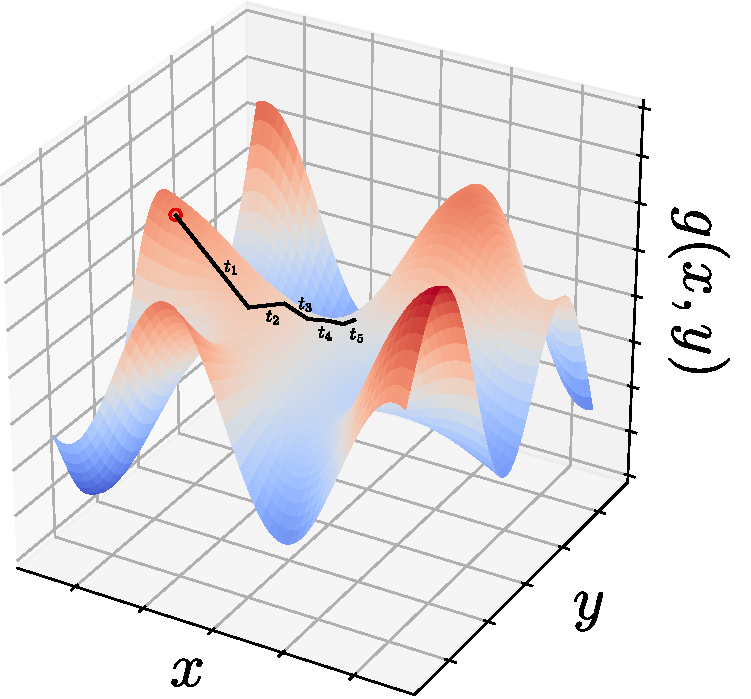
\includegraphics[width=0.8\textwidth]{Chapter3/func_exam.pdf}
    \caption{Gradient descent on function g.}
    \label{fig:grad_desc}
\end{figure}

\subsubsection{Stochastic Gradient Descent}

Another popular algorithm is Stochastic Gradient Descent (SGD) that is a stochastic approximation of Gradient Descent.
Instead of calculating $J(\theta)$ as an average between all the samples, the gradient update step is done once per sample.
It calculates an approximation of the gradient and updates the parameters $\theta_i$ with every sample.
Algorithm \ref{algo:sgd} describes SGD

\begin{algorithm}[H]
    \DontPrintSemicolon
    \SetAlgoLined
    \KwResult{Function minimum}
    \While{An approximate minimum is not obtained} {
        Randomly shuffle examples in the training set\;
        \For{i = 1,2,..., m} {
            $\theta_i = \theta_i - \alpha \nabla J_i(\theta)$\;
        }
    }
    \caption{SGD algorithm.}
    \label{algo:sgd}
\end{algorithm}

The gradient approximation for SGD is much faster to compute, however, since it is a noisy estimate of the gradient,
SGD may need more steps to converge to a local minimum.

\subsubsection{Mini-Batch Gradient Descent}
Finally, Mini-Batch Gradient Descent combines the idea from Gradient Descent and SGD.
It computes the gradient using more than one training example, called a \textit{mini-batch}, at each step. It may result
in smoother convergence and the code can be accelerated by making use of vectorization.

\section{Back Propagation}
\label{subsec:back_prop}

We have seen how a few gradient-based optimization algorithms work. 
To minimize the cost function we need to compute the partial derivatives of the cost function w.r.t. 
to each weight of the neural network. Calculating these partial derivatives manually would be computacionally
infeasible for large networks.
In deep neural networks, by using the chain rule, we can calculate the partial derivatives in an efficient and
compact way.

Backpropagation is an algorithm that computes the gradients of the loss function w.r.t. each input from the network.

% % Gradient image

% Therefore numerical gradient computation is an important step in deep learning.

\chapter{Deep Reinforcement Learning}
\label{chap:deep_rl}
%The previous two chapters described the background for RL and DL. In this chapter, we will see 
%how these two fields are combined in powerful state-of-the-art algorithms for solving complex reinforcement learning problems.
%In this work, we use all the algorithms presented in this chapter.

The previous chapter described a summarized background for RL concepts and classical algorithms. This chapter aims to go deeper towards the techniques we are actually going to use in this work. First, we must build the background for Neural Networks (NN) and Multi Layer Perceptrons (MLP), which are commonly used as policy and value function approximations in modern RL algorithms. Then, we will present two state of the art RL techniques which we plan to use in our problem.

\section{Neural Networks}

Neural Networks are mathematical structures that receive inputs and calculate outputs. In this sense, can be described as a mathematical technique to fit very complex and non-linear functions.

Also known as Multi Layer Perceptron (MLP), it has a multiple layer architecture, where each layer is composed by several nodes called neurons. These nodes, in an analogy to human brain neurons, are still mathematical units which receives some numerical inputs and outputs one single number. All of these mathematical units make use of a specific set of parameters.

\subsection{Representation}

Regarding the representations and notations used for NN, we can describe its basic elements consisting of inputs, outputs, parameters and activate functions.

For each one of the $m$ training examples, we define the input $x^{(i)}$, corresponding to the $i$th example, as a n-dimensional feature column vector, so with dimensions $(n,1)$. It is also called the input layer, with $0$ index, and also represented as $a^{[0](i)}$ with dimensions $(n^{[0]},1)$. Moreover, we also define the final expected output for each training example, given by the vector $y^{(i)}$ with dimensions $(n_F,1)$.

For each layer $l$, also called hidden-layers, with $1<l<L$ in a total of $L$ layers, we have a specific structure:
\begin{itemize}

\item
	The layer $l$ has a total of $n^{[l]}$ hidden units, each $j$th unit receives all the inputs $a^{[l-1](i)}$ from layer $l-1$, and output a scalar $a^{[l](i)}_j$. The total output of the layer is then composed by all hidden units outputs, given by the vector $a^{[l](i)}$, with dimensions $(n^{[l]},1)$.
	
\item
	Each $j$th hidden unit has a row-vector linear parameter $w^{[l]}_j$ with dimensions $(1,n^{[l-1]})$. The total linear parameters $W^{[l]}$ of the layer is given by all hidden units parameters in a $(n^{[l]},n^{[l-1]})$ matrix.
	
\item
	Each $j$th hidden unit also has a scalar bias-parameter given by $b^{[l]}_j$, and all units bias-parameters compose the layer bias vector $b^{[l]}$, with dimensions $(n^{[l]},1)$
	
\item
	The layer also has a specific activation function $g^{[l]}(z)$, which can assume different mathematical functions, such as the \textit{sigmoid} function, the \textit{tanh} function, and, the \textit{ReLU} function, shown in Equation \eqref{eq:common_activation_functions}.

\begin{equation}
sigmoid(z) = \frac{1}{1+e^{-z}} \text{ ; } tanh(z) = \frac{e^z - e^{-z}}{e^z + e^{-z}} \text{ ; } ReLU(z) = max(z,0)
\label{eq:common_activation_functions}
\end{equation}

\end{itemize}

All these elements of the layer are related through the update Equations \eqref{eq:linear_update_nn} and \eqref{eq:non_linear_update_nn}, which, for each layer $l$, receives the previous layer output $a^{[l-1](i)}$ and generates the current layer output $a^{[l](i)}$. The Figure \ref{fig:nn_basic_architecture} illustrates this representation for a shallow one hidden-layer NN.

\begin{align}
z^{[l](i)} = W^{[l]}a^{[l-1](i)} + b^{[l]}
\label{eq:linear_update_nn}
\\
a^{[l](i)} = g^{[l]}(z^{[l](i)})
\label{eq:non_linear_update_nn}
\end{align}

\begin{figure}[H]
    \centering
    \includegraphics[width=0.6\textwidth]{Chapter4/neuralnet.pdf}
    \caption{Shallow Neural Network Architecture.}
    \label{fig:nn_basic_architecture}
\end{figure}

One last basic definition for NN is the cost function $J(W^{[1]},b^{[1]},...,W^{[L]},b^{[L]})$. The cost function basically measures how good our estimator is to our dataset. The lower the cost function, the less error we obtain when predicting the desired function. Therefore, it represents the target function to be minimized, with respect to all the parameters used in the NN $\{ W^{[1]},b^{[1]},...,W^{[L]},b^{[L]} \}$.

It is possible to employ several different cost functions according to each specific problem. However, we can mention the most common ones, that are the Quadratic Cost, given by Equation \eqref{eq:quadratic_cost}, and the Cross-Entropy Cost, given by Equation \eqref{eq:cross_entropy_cost}.

\begin{equation}
J(W^{[1]},b^{[1]},...,W^{[L]},b^{[L]}) = \frac{1}{m} \sum_{i=1}^{m}{\sum_{j=1}^{n^{[L]}}{ (y_j^{(i)} - a_j^{[L](i)})^2 }}
\label{eq:quadratic_cost}
\end{equation}

\begin{equation}
J(W^{[1]},b^{[1]},...,W^{[L]},b^{[L]}) = \frac{1}{m} \sum_{i=1}^{m}{\sum_{j=1}^{n^{[L]}}{ \left[ y_j^{(i)}\log{a_j^{[L](i)}} - (1-y_j^{(i)}) \log{ (1 - a_j^{[L](i)}) } \right] }}
\label{eq:cross_entropy_cost}
\end{equation}

% describe:
% para cada exemplo de 1 a m, temos um vetor de input x (n[0],1)
% para cada camada de 1 a L, temos:
%			 n[l] hidden units,
%			 uma matriz de parametros W (n[l],n[l-1])
%			 e um vetor de bias b (n[l],1)
% activation functions
% cost function

\subsection{Vectorization}

The previous equations are capable of fully defining update rules for any MLP, however, in order to avoid the naively computation over each training example, and therefore reach more efficient algorithms exploring the use of parallelization in modern GPUs architectures, we must introduce a vectorization notion.

Let's first define the $X$ matrix as the concatenation of each training example $x^{(i)}$ composing its columns, as shown in Equation \eqref{eq:vectorization_concatenation_X}. The matrix $X$ now assumes the dimensions $(n^{[0]},m)$.

\begin{equation}
X = 
\begin{bmatrix}
\vdots & \vdots &  & \vdots \\
x^{(1)} & x^{(2)} & \dots & x^{(m)} \\
\vdots & \vdots &  & \vdots
\end{bmatrix}
\label{eq:vectorization_concatenation_X}
\end{equation}

In this sense, we can analogously define the matrices $A^{[l]}$ and $Z^{[l]}$, as a concatenation of the values for each example $a^{[l](i)}$ and $z^{[l](i)}$, described in Equation \eqref{eq:vectorization_concatenation}. The matrices $A^{[l]}$ and $Z^{[l]}$ now assume the dimensions $(n^{[l]},m)$.

\begin{equation}
A^{[l]} = 
\begin{bmatrix}
\vdots & \vdots &  & \vdots \\
a^{[l](1)} & a^{[l](2)} & \dots & a^{[l](m)} \\
\vdots & \vdots &  & \vdots \\
\end{bmatrix}
\text{ }
Z^{[l]} = 
\begin{bmatrix}
\vdots & \vdots &  & \vdots \\
z^{[l](1)} & z^{[l](2)} & \dots & z^{[l](m)} \\
\vdots & \vdots &  & \vdots \\
\end{bmatrix}
\label{eq:vectorization_concatenation}
\end{equation}

The update equations for each layer, in the vectorized representation, is therefore modified and given by the Equations \eqref{eq:linear_update_nn_vectorized} and \eqref{eq:non_linear_update_nn_vectorized}.

\begin{align}
Z^{[l]} = W^{[l]}A^{[l-1]} + b^{[l]}
\label{eq:linear_update_nn_vectorized}
\\
A^{[l](i)} = g^{[l]}(Z^{[l]})
\label{eq:non_linear_update_nn_vectorized}
\end{align}

\subsection{Forward Propagation}

Given all the definitions of the basic structures of a NN and the main calculations involved, we can derive the algorithm for the forward propagation. The forward Propagation algorithm consists in: given all the dataset composed by the matrix $X$, compute all layers outputs $A^{[l]}$ and $Z^{[l]}$, including the final layer and the final output of the NN, which are $A^{[L]}$ and $Z^{[L]}$.

\begin{algorithm}[H]
    \DontPrintSemicolon
    \SetAlgoLined
    \For{ $l$ = $1$, ..., $L$ }{
        $Z^{[l]} = W^{[l]} A^{[l-1]} + b^{[l]}$\;
        $A^{[l]} = g^{[l]}(Z^{[l]})$\;
        cache $Z^{[l]}$ and $A^{[l]}$\;
    }
    \Return{$A^{[L]}$}
    \caption{Forward Propagation}
    \label{algo:forward_propagation}
\end{algorithm}

\subsection{Backward Propagation}

The ultimate goal in Supervised Learning is minimizing the cost function. For this purpose, one of the most famous optimization techniques used is gradient descent. However, in order to make use of gradient descent, we must compute the derivatives of the cost function with respect to all the parameters $W^{[1]}, b^{[1]}, ..., W^{[L]}, b^{[L]}$. The notation we are going to use for these partial derivatives is given in Equations from \eqref{eq:partial_derivatives_notation_first} to \eqref{eq:partial_derivatives_notation_final}.

\begin{align}
\frac{\partial J(\theta)}{\partial W^{[l]}} = dW^{[l]}
\label{eq:partial_derivatives_notation_first}
\\
\frac{\partial J(\theta)}{\partial b^{[l]}} = db^{[l]} \\
\frac{\partial J(\theta)}{\partial A^{[l]}} = dA^{[l]} \\
\frac{\partial J(\theta)}{\partial Z^{[l]}} = dZ^{[l]}
\label{eq:partial_derivatives_notation_final}
\end{align}

Finding a closed expression for each partial derivative would be a massive analytical work, hence an elegant solution is to employ a iterative algorithm called Backward Propagation, or Backpropagation. The main idea involved in this algorithm is computing each layer output derivative from the next layer output derivative $dA^{[l]}$ and the cached data $A^{[l-1]}$ and $Z^{[l]}$ from the forward propagation algorithm. The Backpropagation algorithm is then given in Algorithm \ref{algo:backward_propagation}.

\begin{algorithm}[H]
    \DontPrintSemicolon
    \SetAlgoLined
    $dA^{L} = \sum_{i=1}^m{\frac{-y^{(i)}}{a^{[L](i)}} + \frac{(1-y^{(i)})}{(1-a^{[L](i)})}}$\;
    \For{ $l$ = $L-1$, ..., $1$ }{
        input $dA^{[l]}$ and cached values $A^{[l-1]}$ and $Z^{[l]}$\;
        $dZ^{[l]} = dA^{[l]} * g'^{[l]}(Z^{[l]})$(element-wise multiplication)\;
        $dW^{[l]} = \frac{1}{m} dZ^{[l]} A^{[l-1]T}$\;
        $db^{[l]} = \frac{1}{m}$ sum over rows of $dZ^{[l]}$\;
        $dA^{[l-1]} = W^{[l]T}dZ^{[l]}$\;
    }
    \Return{($dW^{[1]}, db^{[1]}, ..., dW^{[L]}, db^{[L]}$)}
    \caption{Backward Propagation}
    \label{algo:backward_propagation}
\end{algorithm}

Finally, by making use of the partial derivatives already computed, we can employ the classical Gradient Descent, described in Algorithm \ref{algo:gradient_descent}. Notice that, until convergence, we update all the parameters by the derivatives computed from all the training examples in each step, consisting in the Batch Gradient Descent.

\begin{algorithm}[H]
    \DontPrintSemicolon
    \SetAlgoLined
    Initialize $W^{[1]},b^{[1]},...,W^{[L]},b^{[L]}$ with random values near $0$\;
    \While{ An approximate minimum is not obtained }{
	    Forward Propagation()\;
	    Backward Propagation()\;
   		\For{ $l$ = $1$, ..., $L$ }{
   			$W^{[l]} = W^{[l]} - \alpha dW^{[l]}$\;
   			$b^{[l]} = b^{[l]} - \alpha db^{[l]}$\;
        }
    }
    \Return{($W^{[1]}, b^{[1]}, ..., W^{[L]}, b^{[L]}$)}
    \caption{Gradient Descent}
    \label{algo:gradient_descent}
\end{algorithm}

%\subsection{Optimizations}

\section{Trust Region Policy Optimization}

Given all the RL and NN background necessary, we will introduce two state of the art techniques combining both fields.

The intersection relies on the fact that we need complex non-linear functions to efficiently estimate policies and value-functions. Therefore, the most common used structure for this approximation is MLP. Aiming also to fit stochastic policies distributions in continuous action spaces, we define our policy $\pi_{\theta}(s|a)$ by a normal distribution $\mathcal{N}(\mu,\sigma)$, where the mean $\mu$ and log standard deviation $\sigma$ are outputs of a neural network \cite{TRPO}.

Moreover, in order to work with continuous action spaces, we must employ policy search or actor-critic methods. The classic vanilla policy gradient methods, however, bring some limitations that are handled in the recent techniques. We can cite the main limitation as the vulnerability to the step size in the optimization procedure. This fact brings even bigger impacts due to the non-stationary nature of the input data, which means that a small error in the policy update affects the visitation distribution and consequently the future policy updates.

%The Trust Region Policy Optimization tries to address this limitation. TRPO consists in an on-policy approach that transforms a RL problem into an optimization problem, making policy $\pi$ improves through REINFORCE \cite{REINFORCE} by computing an ascent direction based on data sampled from $\pi$. However, the novel idea introduced by this algorithm is limiting the policy step size to lie within a so called trust region, and thus avoid divergence.

The Trust Region Policy Optimization tries to address this limitation. The novel idea introduced by this algorithm is limiting the policy step size to lie within a so called trust region, and thus avoid divergence. This trust region is computed through the Kullback-Leibler (KL) divergence. The KL divergence is basically a measure of the deviation between two probability distributions, and it is defined as the relative entropy between two continuous random variables $P$, $Q$. Let $p(x)$ and $q(x)$ be the probability density functions of $P$ and $Q$ respectively, the KL divergence, $KL[P,Q]$, is then given by equation \ref{eq:KL_divergence}.

%The trust region is computed through the Kullback-Leibler (KL) divergence. The KL divergence is basically a measure of the deviation between two probability distributions, and it is defined as the relative entropy between two continuous random variables $P$, $Q$. Let $p(x)$ and $q(x)$ be the probability density functions of $P$ and $Q$ respectively, the KL divergence, $KL[P,Q]$, is then given by equation \ref{eq:KL_divergence}.

\begin{equation}
KL[P,Q] = \int_{-\infty}^{\infty}{p(x)\log{\frac{p(x)}{q(x)}}}
\label{eq:KL_divergence}
\end{equation}

TRPO therefore limits the policy gradient step size by applying a KL based constraint \eqref{eq:TRPO_2} to an optimization problem on a slightly modified cost function \eqref{eq:TRPO_1}. The overall algorithm is iteratively, we run episodes and collect data from $\pi_{\theta_{old}}$, compute $\pi_{\theta}$ from the optimization problem and then update $\pi_{\theta_{old}} \leftarrow \pi_{\theta}$. This method is described in Algorithm \ref{algo:TRPO}.

%consists in a constrained optimization problem, given by equations

\begin{align}
\underset{\theta}{\textrm{maximize }} \mathbb{\hat{E}}_{s_t,a_t \sim \pi_{\theta_{old}} } \left[ \frac{\pi_{\theta}(a_t|s_t)}{
\pi_{\theta_{old}}(a_t|s_t)}\hat{A}_t \right]
\label{eq:TRPO_1}
\\
\textrm{subject to } \mathbb{\hat{E}}_{s_t,a_t \sim \pi_{\theta_{old}} } \left[ KL[\pi_{\theta_{old}},\pi_{\theta}(.|s_t)] \right] \leq \delta
\label{eq:TRPO_2}
\end{align}

\begin{algorithm}[H]
    \DontPrintSemicolon
    \SetAlgoLined
    \For{ iteration = $1$, $2$, ... }{
    	Run policy for N trajectories\;
    	Estimate advantage function $\hat{A}(.)$ at all $n$ timesteps\;
    	$\underset{\theta}{\textrm{maximize }} \sum_{n=1}^{N} {\frac{\pi_{\theta}(a_n|s_n)}{\pi_{\theta_{old}}(a_n|s_n)}\hat{A}_n }$\;
    	$\textrm{subject to } \overline{KL}[\pi_{\theta_{old}},\pi_{\theta}(.|s_t)] \leq \delta$\;
    	$\pi_{\theta_{old}} \leftarrow \pi_{\theta}$\;
    }
    \Return{$\pi_{\theta}$}
    \caption{TRPO}
    \label{algo:TRPO}
\end{algorithm}

In this algorithm, we must compute an estimate for the advantage function $\hat{A}_t$. The advantage function is given by $A(s_t,a_t) = Q(s_t,a_t) - V(s_t)$, and it is basically the standard critic function $Q(s_t,a_t)$ subtracted by a unbiased baseline $V(s_t)$ (state-value function) in order to reduce variance. For solving the constrained optimization problem, the conjugate gradient method is generally used.

TRPO presents a great improvement under data efficiency and convergence properties. However, it has a great computational cost, and its implementation through conjugate gradients can be relatively complicated \cite{PPO}.

\section{Proximal Policy Optimization (PPO)}

The Proximal Policy Optimization \cite{PPO} is a recent technique that follows a similar approach used for TRPO, which consists in solving an optimization problem by computing an update at each step that minimizes the cost function while ensuring a relatively small deviation from the previous policy. However, the great breakthroughs introduced are enhancements in the ease of implementation and the ease of hyperparameters tuning, while achieving an even better performance.

The main idea behind TRPO is to use an adaptive KL penalty to control the change of the policy at each iteration. PPO introduces a novel objective function, which intrinsically address this constraint in a first-order optimization.

Let $r_t(\theta)$ be the ratio between the new and old policy, given by the Equation \eqref{eq:def_r_t}, the PPO's objective function is then described by the Equation \eqref{eq:PPO_objective_function}.

\begin{equation}
r_t(\theta) = \frac{\pi_{\theta}(a_t|s_t)}{\pi_{\theta_{old}}(a_t|s_t)}
\label{eq:def_r_t}
\end{equation}

\begin{equation}
L(\theta) = \mathbb{\hat{E}}_t \left[ min(r_t(\theta)\hat{A}_t, clip(r_t(\theta),1-\epsilon,1+\epsilon)\hat{A}_t) \right]
\label{eq:PPO_objective_function}
\end{equation}

In Equation \eqref{eq:PPO_objective_function}, $\theta$ is the policy parameters, $\mathbb{\hat{E}}_t$ is the empirical expectation over all $t$ timesteps, $\hat{A}_t$ is the estimate for the advantage function, as already described, $\epsilon$ is a new hyperparameter, and finally the clip function is explained in Equation \eqref{eq:clip_function}.

\begin{equation}
clip(x,min,max) = \begin{cases}
        min, & \mbox{if } x < min \\
        x, & \mbox{if } min \leq x \leq max \\
        max, & \mbox{if } x > max
        \end{cases}
\label{eq:clip_function}
\end{equation}

PPO does not need complex conjugate gradient techniques, and can be solved with classical stochastic gradient descents. Besides, it has displayed the best performance on continuous control tasks, even compared to TRPO, it also allows parallel implementations and it is very data efficient.

%ease of implementation, sample complexity, and ease of tuning
%compute an update at each step that minimizes the cost function while ensuring the deviation from the previous policy is relatively small.
%TRPO uses an apdtive KL penalty to control the change of the policy at each iteration
%PPO uses a novel objective function which already address this contraint
%present the objective function
%doesnt need complex conjugate gradient techniques, can be solved with the standard stochastic gradient descent
%it has displayed the best performance on continuous control tasks, even compared to TRPO, allows parallel implementations and is very data efficient



\chapter{Methodology}
\label{chap:method}

This chapter will describe all the development tools and infrastructure used. Besides, it includes a brief description of the kick engine which this work was based on, and the set of metrics we will use to evaluate our learning results and performance.

\section{Tools}

\subsection{C++}

C++ is a general purpose programming language that is highly efficient and flexible. It is famous for introducing a oriented-based paradigm with high performance processing, by allowing low-level memory manipulations and a machine compiled syntax \cite{C++}.

The ITAndroids Soccer3D base code was already built in C++, and therefore any additional work made which interacts with the soccer simulation server was also developed in C++ in order to integrate seamlessly with the codebase. For this work, we used version 14, which is one of the most recent and stable standardized version.

\subsection{Python}

Python is an interpreted general purpose high-level programming language \cite{Python}. It has a easy-to-read syntax closely resembling pseudo-code, which makes easier and quicker to prototype new ideas. For this reason, Python was widely chosen as one of the most used programming languages in the deep learning community, and many of the AI frameworks and reference algorithms we used was developed in or have a great integration with Python.

For this work, we chose version 3.5, since it is one of the most recent and stable versions, and also is used by other frameworks.

\subsection{Protocol Buffers}

Protocol Buffers is a multiplatform library for serializing structured data that supports multiple programming languages \cite{ProtoBuf}. It is very useful for developing uncoupled client-server applications that communicate using a simple and flexible API. For these reasons, we chose Protocol Buffer as the client-server API.

\subsection{OpenAI Baselines}

OpenAI Baselines is a set of high-quality implementations of reinforcement learning algorithms open sourced by OpenAI. The purpose is to provide algorithms which will make it easier for the research community to replicate, refine, and identify new ideas, and therefore create good baselines to build research on top of. \cite{baselines}

\begin{figure}[H]
    \centering
    
\includegraphics[width=0.3\textwidth]{Chapter5/openai_logo.jpg} 
    \caption{OpenAI Logo.}
    \label{fig:openai_logo}
\end{figure}

Besides the OpenAI Baselines, we also used the OpenAI Gym, which consists of a toolkit for running reinforcement learning algorithms in different environments \cite{OpenAIGym}. It allows testing and benchmarking RL algorithms by providing a standardized set of environments. Figure \ref{fig:openai_envs} illustrates a few example environments from OpenAI Gym.

\begin{figure}[H]
    \centering
    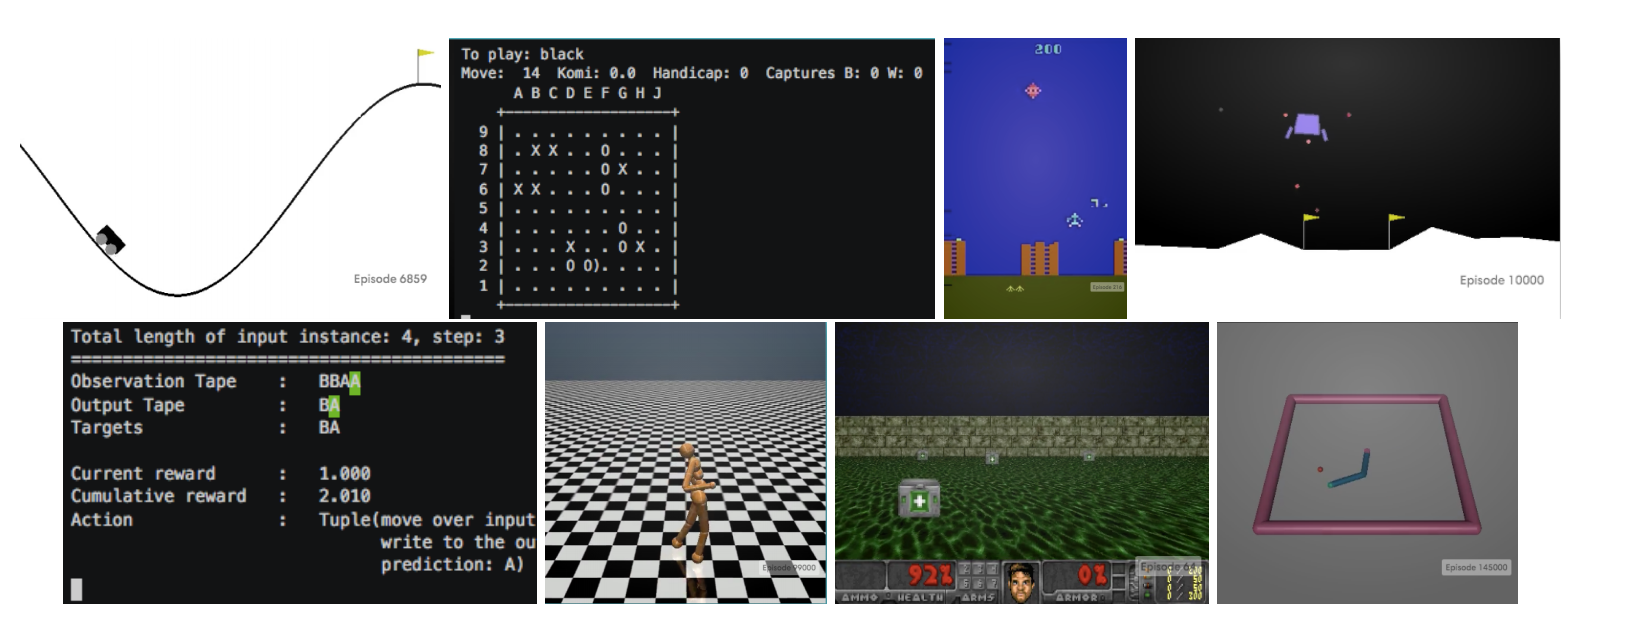
\includegraphics[width=0.85\textwidth]{Chapter5/openai_env.png} 
    \caption{OpenAI Gym environments, extracted from \cite{OpenAIGym}.}
    \label{fig:openai_envs}
\end{figure}

For these reasons, we made use of the PPO implementation from OpenAI Gym, and adapted the Gym environment to work for the Soccer3D Simulation. This process is further described in the next chapter.

\subsection{Tensorflow}

TensorFlow is an open source software library for numerical computation using data flow graph \cite{TensorFlow}. It is greatly used for machine learning applications due to its highly efficient implementations of gradient computation and optimization, by introducing parallelization and making use of specialized hardware instructions like SSE and GPU. TensorFlow is also used by OpenAI Baselines, in its RL algorithms implementations.

TensorFlow also provides several useful tools, such as TensorBoard, which consists in a visualization dashboard very helpful for debugging and plotting.

\subsection{Intel AI DevCloud}
\label{sec:devcloud}

Intel AI DevCloud is a cloud hosted hardware and software platform available to developers, researchers and startups to learn, sandbox and get started on their Artificial Intelligence Projects \cite{devcloud}. It provides access to Intel Xeon Scalable Processors, and therefore a powerful infrastructure for running optimizations and machine learning algorithms.

Intel is also a sponsor of the ITAndroids team, and provided extended use of DevCloud for this project.

\begin{figure}[H]
    \centering
    
\includegraphics[width=0.3\textwidth]{Chapter5/intelai_logo.jpg} 
    \caption{Intel AI Logo.}
    \label{fig:intelai_logo}
\end{figure}

\section{Simulation Interface}

This work's simulation environment is the \textit{SimSpark} simulator \cite{Simspark}. It makes use of the Open Dynamics Engine \cite{ODE} for rigid body dynamics and collision detection, and also allows multi-agent simulations in a single environment, hosting up to two teams of eleven humanoid robots to play against each other.

The \textit{SimSpark} server also introduces noise, breaking the reproducibility of events and turning the problem more realistic. Consequently, this process fairly increases the challenge of the learning problem.

For this work, we also used \textit{RoboViz}, a publicly available visualization tool created by Justin Stoecker \cite{RoboViz} that allows several improvements over the default visualization tool. Figure \ref{fig:roboviz_game} shows a typical game scene inside \textit{RoboViz}.

\begin{figure}[H]
    \centering
    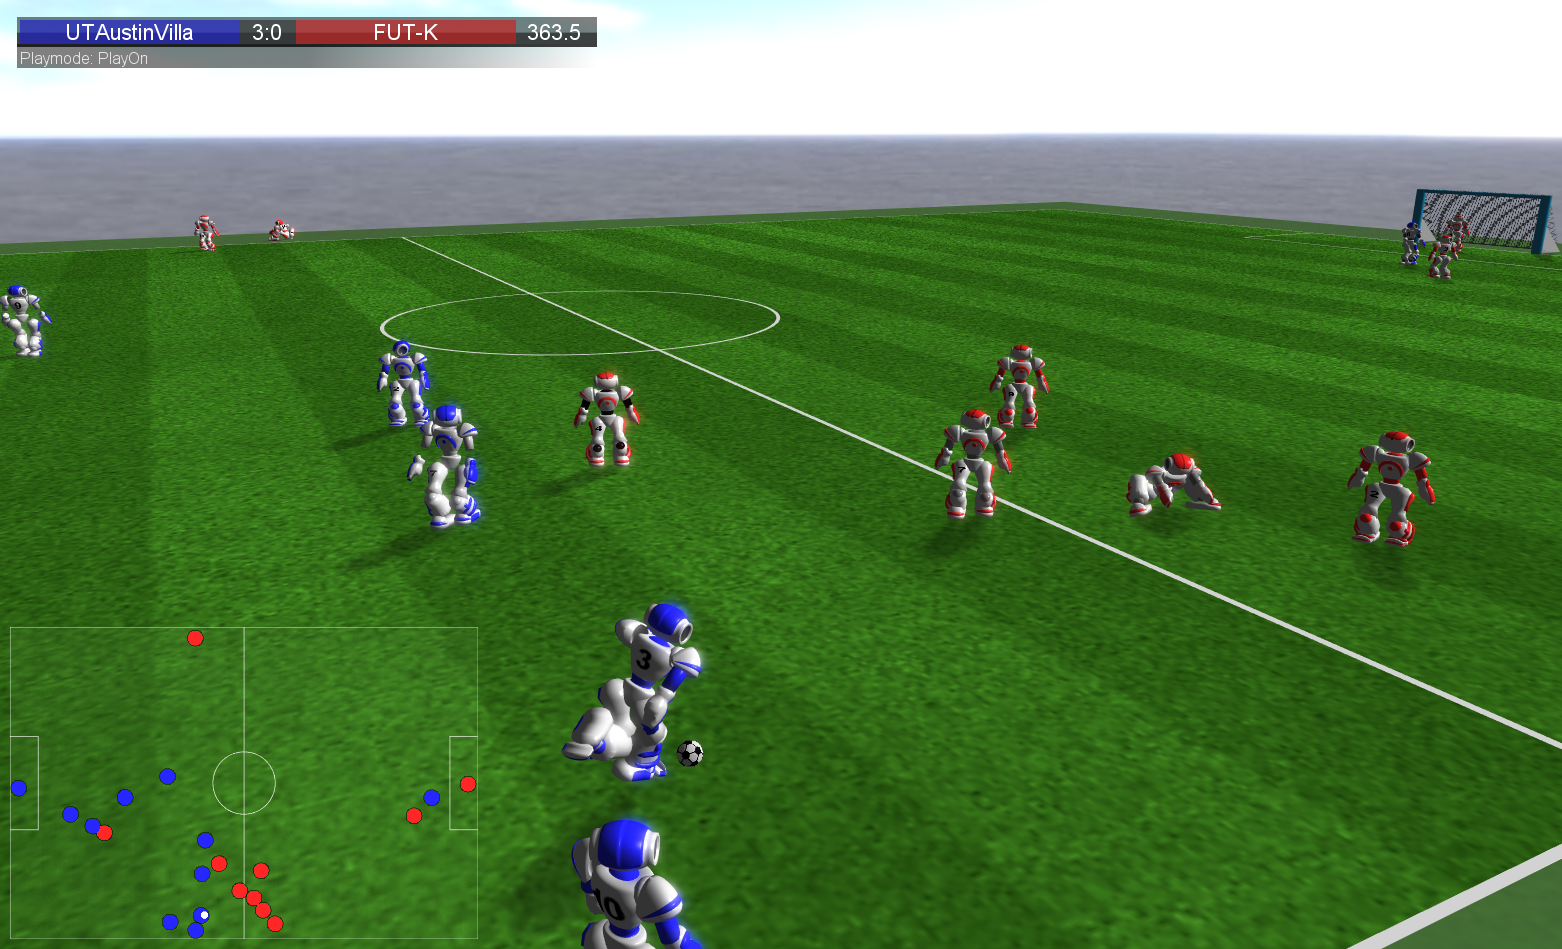
\includegraphics[width=0.8\textwidth]{Chapter5/sim3d.png} 
    \caption{Soccer match in \textit{SimSpark} simulation environment.}
    \label{fig:roboviz_game}
\end{figure}

The agent in \textit{SimSpark} is a simulated version of the Nao humanoid robot, manufactured by SoftBank Robotics \cite{NaoRobot}, presenting 22 joints and therefore offering 22 degrees of freedom. At each timestep, the simulated agent communicates with the simulator using TCP connections, sending the desired velocities commands for all joints, followed by the server simulation step, which takes $\Delta t = 0.02s$. The server step process all the physical dynamics, and send back to the agent its joints positions with other informations. \cite{SimSparkEffectors}.

\section{ZMP Kick Engine}
\label{sec:ZMPkick}

The ZMP Kick Engine is an algorithm that performs a complete kicking motion based on the Zero Moment Point dynamic. This engine calculates the joints positions during all the movement and feed this data to PID controllers at each joint to compute the commanded velocities actually sent to the server. In this work, we are not specifically interested in the Kick Engine itself, but it is important to understand some low level aspects of this base movement, since it has a big influence in the learned kick behavior we are interested to develop.

The Zero Moment Point (ZMP) is a popular concept in the humanoid literature \cite{ZMP}, and can be thought as the dynamic version of the center of mass (CoM) due to the following stability criterion: a biped is dynamically stable at a given time instant if the ZMP is inside the support polygon, which consists of a convex hull of all contact points on the ground \cite{ZMP}. Moreover, by using the ZMP concept and the Linear Inverted Pendulum Model \cite{Kajita} to approximate the robot dynamics, the engine analytically computes a CoM trajectory which keeps the robot dynamically stable during the kick movement. Finally, this CoM trajectory is translated into joint positions by employing Inverse Kinematics.


% Moreover, the engine translates the ZMP position control into joints positions commands by approximating the robot dynamics using the Linear Inverted Pendulum  Model \cite{Kajita}.

The ZMP Kick engine is fully described at \cite{MestradoManga}, but can be briefly summarized by its 5 phases enumerated below. Figure \ref{fig:kicking_phases} illustrates all these 5 steps.

\begin{itemize}
\item Phase A: the robot moves the ZMP to the center of the support foot to allow the kicking foot to be taken off the ground without the robot losing balance.

\item Phase B: the kicking foot is moved backwards at the same time that is taken off the ground. Therefore, preparing to kick the ball.

\item Phase C: the robot kicks the ball, performing a trajectory for the kicking foot with a horizontal continuous speed.

\item Phase D: in this phase, the kicking foot should do the inverse that was done in Phase B, moving the foot from the air to the ground.

\item Phase E: the robot finally goes back to the stand position, moving the ZMP to the torso projection on the ground.

\end{itemize}

\begin{figure}[H]
    \centering
    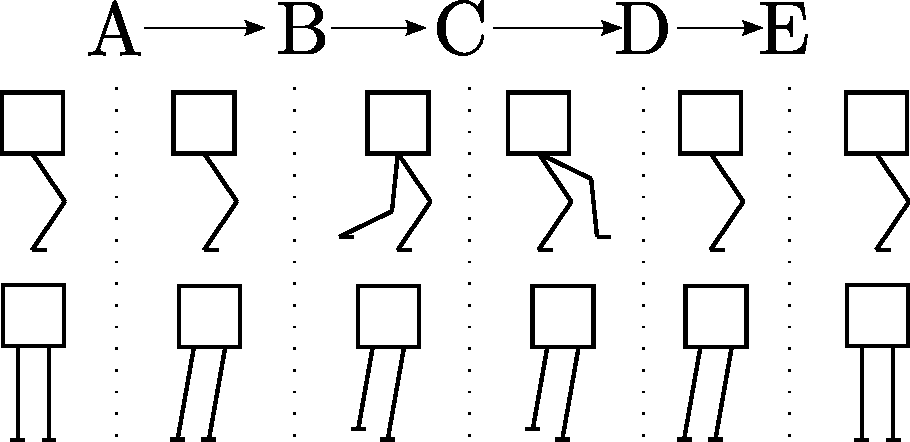
\includegraphics[width=0.7\textwidth]{Chapter5/kicking_phases.pdf} 
    \caption{Phases for a kick with right leg. The upper row shows poses looked from the right of the robot, while the lower one presents poses looked from the front. Extracted from \cite{MestradoManga}.}
    \label{fig:kicking_phases}
\end{figure}


\section{Metrics}
\label{sec:metrics}

When working on some reinforcement learning tasks, it is very important to previously define some metrics to assess the learning performance during the training stages. Raising this information, we can evaluate the techniques, identify the problems and consider improvements. In this work, we focused on two main metrics:

\begin{itemize}
\item \textbf{Episode accumulated reward:} Maximizing the episode return is the ultimate goal of RL, and therefore it is the most obvious performance indicator, providing a very good sense of how well the agent's actions are doing.

\item \textbf{Data efficiency:} A quantitative measure of how long, or how much data, an agent takes to learn a good behavior.
\end{itemize}

We calculate all these metrics in an offline manner, by logging all the state and action information from the agent during the training procedure.




\chapter{Learning Kick Behaviors}
\label{chap:contributions}

The major contribution of this work is providing a task modeling and setup for learning humanoid soccer movements in the RoboCup Soccer3D domain using reinforcement learning frameworks. We also introduce the deep mimic approach for this class of problems and a specific curriculum to learn, as well as several implementation considerations, manually tunned and developed after a few processes iterations.

\section{Environment and Implementation}

As previously mentioned in section \ref{chap:method}, this work used the RL algorithms implementations from the OpenAI baselines repository \cite{baselines}. More specifically, the high-quality implementation of PPO. Not implementing the DRL algorithms from scratch made it much easier to test, iterate, improve and focus on developing the agent experiments.

The PPO implementation on Baselines was adapted to change the communication with the OpenAI Gym environments to communicate with the Soccer3D agent, maintaining the same function protocols.

The framework used to integrate the baselines code with new experiments, flexible to develop, in the Soccer3D domain was already built in the work \cite{TGMuzio}. This framework can be basically described by its two main modules, each one running as a separate process and communicating through Protocol Buffers.

\begin{itemize}
\item \textbf{Learning Client:} Process that runs the reinforcement learning algorithms and makes remote procedure calls (RPCs) to the server, exchanging state/action information with the soccer agent. This module was implemented in Python 3.5 and TensorFlow, using OpenAI Baselines implementations.

\item \textbf{Soccer Agent:} The simulated agent which interacts with \textit{SimSpark} and with the learning client, executing the learning experiments. This module was implemented in C++ and uses the ITAndroids Soccer Simulation 3D code base.
\end{itemize}

As already commented, the API between server and client uses Protocol Buffers, with the exchange of RPCs containing the standard state, action, reward and end of episode information used in OpenAI Gym. An illustration of this framework follows in the diagram presented in Figure \ref{fig:RL_framework}. For details, please refer to \cite{TGMuzio}.

\begin{figure}[H]
    \centering
    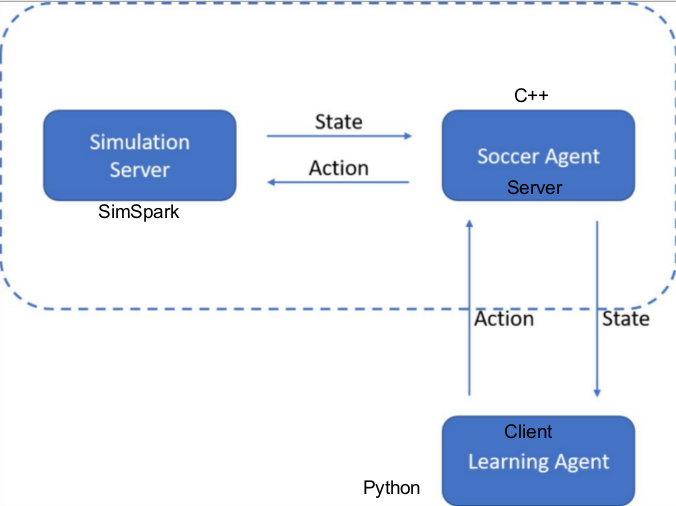
\includegraphics[width=0.8\textwidth]{Chapter6/architecture.png} 
    \caption{Learning Architecture diagram. Extracted from \cite{TGMuzio}}
    \label{fig:RL_framework}
\end{figure}

\section{Infrastructure}

This work used the Intel AI DevCloud as its main infrastructure to run all learning experiments described below.

The cluster is composed by 10 computation nodes using each one a 24 cores Intel Xeon processor. Furthermore, the experiments setup exploited the parallelization feature of PPO, running up to 12 Soccer Agents per node, besides the Learning Client process, and collecting a total number of samples in the magnitude of 100 million.

\section{Deep Mimic Learning}

The Deep Mimic approach \cite{deepmimic} established a great new paradigm in which this work was based on. It introduces a novel idea of allowing the supply of reference motions from motion capture or hand-authored animation data for style, and then generating goal-directed and physically realistic behavior from those reference motions \cite{deepmimic}.

The basic approach presented for this mission consists in rewarding the agent to produce motions that resemble the reference data, as well as to achieve additional task objectives.

A control policy $\pi (a_t|s_t,g_t)$ maps the state of the character $s_t$ and a task-specific goal $g_t$ to an action $a_t$. The action distribution is gaussian, with fixed covariance and mean given by a neural network. This policy outputs the desired joints positions, which is later translated into torque commands by each joint PD controller.

The overall reward is spitted into the imitation reward, given by $r_I(s_t,a_t)$, and the task-specific reward, given by $r_G(s_t,a_t)$. The final reward is therefore given by Equation \eqref{eq:deep_mimic_reward}.

\begin{equation}
r_t = \omega^I r_t^I + \omega^G r_t^G
\label{eq:deep_mimic_reward}
\end{equation}

The policies are trained with PPO using the clipped surrogate objective, maintaining also a further network for the value function $V_{\psi}(s,g)$.

It is worth mentioning that this work introduces also two novel ideas which significantly increased the robustness and performance of the learning behaviors. 

\begin{itemize}
\item \textit{Reference State Initialization} (RSI) randomly selects a state in which the agent ant its reference actor begins at each episode. In this way, it makes possible to discover high reward future states without the need to learn everything until then, which can be very significant in difficult tasks like backflips.

\item \textit{Early Termination} (ET) finishes the episode when the agent reaches any fruitless condition, such as a fall or joints collision. This process discourage undesirable behaviors and the exploration of bad states, therefore increasing the learning efficiency.
\end{itemize}

\section{Experiments}

In this section, we describe the learning experiments conducted in this work. The ultimate goal is learning a complete behavior capable of kicking the ball towards a planned final distance fed into the input of the policy, however, we started by learning simpler problems. These problems were very useful not only in providing a curriculum learning approach \cite{BengioCurrLearning} and therefore the basements to achieve the final goal, but also helping to validate all the setup, algorithms and to get a better understanding of the problem and the simulation environment limitations.

\subsection{Supervised Kick Learning}

The first tentative of learning a kick behavior was basically learning to imitate the reference kick movement using supervised learning techniques. Therefore, for this experiment, there was no need to use the RL setup or to run a learning agent.

Once the reference movement is deterministic, the neural network used has only one input given by time itself. Two fully-connected hidden layers follow, composed by 512 leaky-relu hidden units each one. Finally, we have a output layer given by 22 linear units, providing position commands for all 22 agent joints.

%For training, we used Adam optimization, applying 5 consecutive optimization cycles with 5000 epochs each one and decreasing the learning rate linearly, applying $10e^{-4}$, $8e^{-4}$, $6e^{-4}$, $4e^{-4}$, $2e^{-4}$ respectively for each cycle.

\subsection{Pure Mimic Learning}

The second checkpoint to achieve was still learning to imitate the reference movement, reaching the best possible precision. However, since we wanted also to validate and test the learning setup, we chose the reinforcement learning approach, using the Proximal Policy Optimization algorithm.

\textbf{State space:} Since the reference movement is deterministic and the commanded actions only depend of the point in time, the 1D observation space consists on the episode timestep solely, given by a multiple of the simulator unit step $0.02s$.

\textbf{Action space:} We decided to restrict the action space to the joints with biggest impact in the kick distance, in order to reduce the learning cost in this task. Therefore, the 6D action space consists on the position commands of the 6 joints on the kicking leg. These position commands are sequentially fed into PID controllers on each joint, in order to generate velocity commands to the motors, which are finally sent to Simspark. It is also worth mention that the other 16 joints will be driven by the ZMP kick engine.

\textbf{Reward signal:} The reward is given by:

\begin{equation}
r_t = -\sum_{j=1}^{6}{|q_t^j-\hat{q}_t^j|^2}
\end{equation}

Where $q_t^j$ and $\hat{q}_t^j$ represent the commanded positions to the j$th$ joint at instant $t$ from the learning agent and from the reference movement, respectively. Therefore, we basically penalize the square difference for all the 6 joints.

The reference movement used was the ZMP kick, described in the previous chapter. We also used a fully-connected NN with two hidden layers, and 512 leaky-relu units each one, followed by an output layer with 6 units.

Besides, in order to simplify the problem in a first moment, we ran everything offline, by comparing the network output with the reference data in a file, without the need to initialize the simulated agent. In this way, we can avoid the physical restrictions involved, and some limitations such as the robot falls, and therefore speeding up the learning process.

Furthermore, the biggest achievement from this task was obtaining a policy network that can also be used as the starting point for the following learning tasks. In this way, it already provides a big learning step in the process of reaching the ultimate goal.

\subsection{Farthest Final Distance Learning}

The following learning task consists in kicking the ball towards the longest possible distance. The purpose is testing the limits of the kick motion, and the deviation the learning process can achieve from the base movement.

We initialized the policy and value-function networks using the resulted ones from the pure mimic task. In this way, the agent already starts knowing a basic behavior for kicking. Therefore, the state and action spaces for this task is the same of the previous task, only requiring a special design for the reward signal.

The reward function was based on the Deep Mimic work \cite{deepmimic}, thus it follows the same format described in \eqref{eq:deep_mimic_reward}. The imitation component will then be given by Equation \eqref{eq:imitation_reward}, while the goal reward is described by Equation \eqref{eq:goal_reward_farthest}.

\begin{equation}
r^I_t = \omega^p r^p_t + \omega^e r^e_t + \omega^c r^c_t
\label{eq:imitation_reward}
\end{equation}

The imitation component in \eqref{eq:imitation_reward} is still composed by three other factors.

The pose reward $r^p_t$ is given by Equation \eqref{eq:position_imitation}, where $q_t^j$ and $\hat{q}_t^j$ represent the commanded positions to the j$th$ joint at instant $t$ from the learning agent and from the reference movement, respectively, and encourages the agent to match the joint orientations of the reference motion at each step.

\begin{equation}
r^p_t = exp \left[ -2 \left( \sum_{j=1}^{6}{|q_t^j-\hat{q}_t^j|^2} \right) \right]
\label{eq:position_imitation}
\end{equation}

The end-effector reward $r_t^e$ is given by Equation \eqref{eq:end_effector_imitation}, where $p_t^e$ and $\hat{p}_t^e$ represent the kicking feet position from the learning agent and reference movement, respectively, and encourages the agent feet to match the positions from the reference movement.

\begin{equation}
r^e_t = exp \left[ -40 \left( |p_t^e-\hat{p}_t^e|^2 \right) \right]
\label{eq:end_effector_imitation}
\end{equation}

At last for imitation, the center-of-mass reward $r_t^c$ is given by Equation \eqref{eq:CM_imitation}, and penalizes the deviation between the agent CM $p_t^c$ and the reference CM $\hat{p}_t^c$.

\begin{equation}
r^c_t = exp \left[ -10 \left( |p_t^c-\hat{p}_t^c|^2 \right) \right]
\label{eq:CM_imitation}
\end{equation}

Finally, we have the goal reward component $r_t^G$ described in Equation \eqref{eq:goal_reward_farthest}. This expression basically encourages the longest distance between ball's final and initial positions, giving a big exponential reward. It is worth to notice that this reward signal is given at each episode timestep, encouraging also the agent to kick the ball as fast as possible.

\begin{equation}
r_t^G = exp \left[ 7 (\text{ballPos - ballInitPos}) \right]
\label{eq:goal_reward_farthest}
\end{equation}

This task was very useful in obtaining a new learned behavior for the first time, starting from the mimic base behavior. Hence, it helped to discover the limitations and particularities of this challenge, improving our overall knowledge about it.

\subsection{Fixed Final Distance Learning}

\subsection{0.8m Fixed Distance}

\subsection{1.5m Fixed Distance}






\chapter{Experiments and Results}
\label{chap:experiments}
According to the methodology described in Chapter \ref{chap:methodology}, we ran a set of experiments
for each of the tasks described in Section \ref{sec:tasks}.
Each experiment is composed of a training phase and a testing phase:

\begin{itemize}
	\item Training phase: The agent is actively learning by sampling data from the simulation server to 
	actively update the parameters of the policy (represented by a neural network).
	\item Evaluation phase: After the initial learning phase, we freeze all the parameters of the agent's 
	policy and evaluate how well it does on the task at hand. 
	We use the metrics describes in Section \ref{sec:metrics} to quantify how well the agent is able to learn the task.
\end{itemize}

In the training phase, we compare the performance for three different deep reinforcement learning algorithms for continuous
control: DDPG, TRPO and PPO.
After the training phase is complete, we evaluate the performance of the learned behaviors and compare them with
classical control behaviors developed by the ITAndroids teams that serve as a performance baseline.

We ran all experiments on a Intel i7-7500U CPU with $4$ logical cores and a GeForce 940MX integrated GPU.
It is important to notice that physical simulation is CPU-bound and, therefore, CPU is the leading
factor of how long the training phase takes to complete.
We will now describe the experiments for each of the tasks.

\section{Humanoid Speed Walker (Warm-Up) Task}

In this domain we are only interested in getting familiar with the environment by learning a very simple task.
We ran PPO once for $10^6$ timesteps with the parameters described in Appendix \ref{chap:appendix_experiment}.
Figure \ref{fig:constant_episode_rew} shows how the average episode returns changes during the training phase of
the algorithm.
Notice how the average episode reward is consistently increasing showing clear signs that the agent is learning how to walk
with the reference speed.

\begin{figure}[ht]
	\centering
	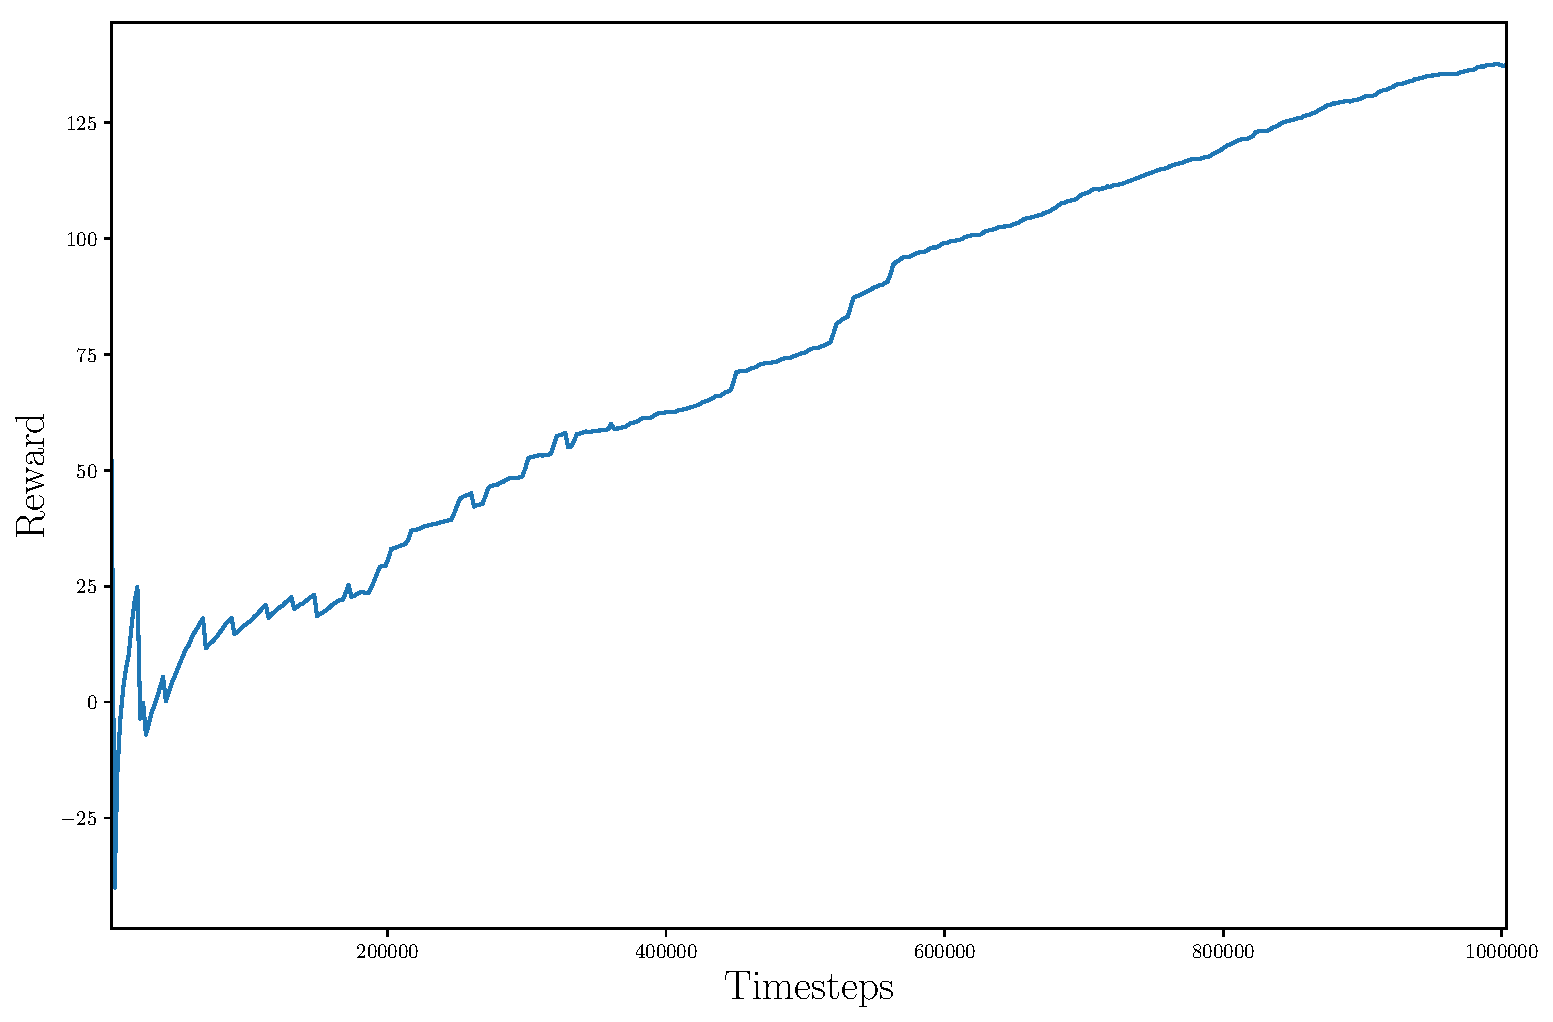
\includegraphics[width=0.9\textwidth]{Chapter7/ep_rew_walker.pdf}
	\caption{Episode Reward for the Constant Speed Walker task trained with PPO.}
	\label{fig:constant_episode_rew}
\end{figure}

In this task, the episode terminates early if the robot falls, therefore, measuring the episode duration
is also a good indicator of how stable the robot's current behavior is.
Figure \ref{fig:constant_episode_len} shows how the episode duration changes during training.
We see that the episode duration increases over training, which means that the agent is progressively
learning how to avoid falling.

\begin{figure}[ht]
	\centering
	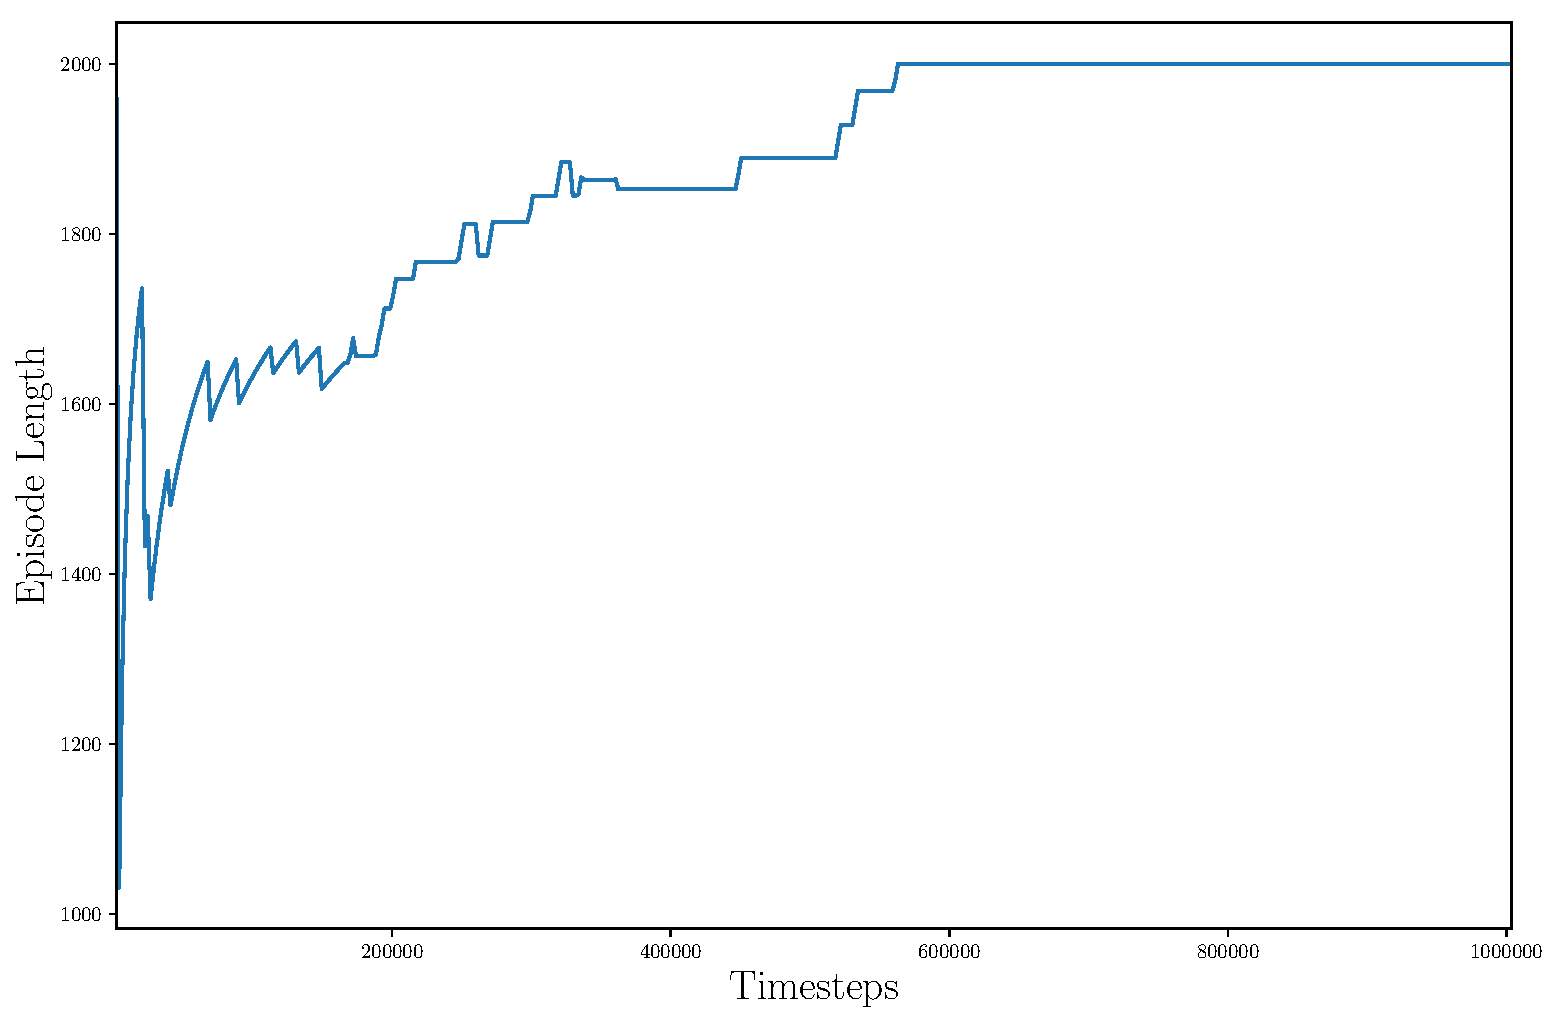
\includegraphics[width=0.9\textwidth]{Chapter7/ep_len_walker.pdf}
	\caption{Episode length for the Constant Speed Walker task with PPO.}
	\label{fig:constant_episode_len}
\end{figure}

Based on the results from Figure \ref{fig:constant_episode_rew} and \ref{fig:constant_episode_len}
we conclude that the agent is effectively learning how to walk with constant speed.
Since this is a very basic task, we chose not to use a baseline agent.

\section{Humanoid Racing Task}

In this domain, we ran PPO, TRPO and DDPG during $10^6$ timesteps with the parameters described in Appendix
\ref{chap:appendix_experiment}. We were interested in comparing the performance of these algorithms in this domain
to see which algorithms performs best in this task.
On average, each experiment took around $3$ hours to run.

Since the algorithms are stochastic and the server simulation is noisy and prone to numerical errors, 
we ran the experiments $5$ times for each algorithm and use the performance mean and standard deviation over all runs
to obtain more statistical significant results.
Figure \ref{fig:racer_episode_rew} depicts the episode rewards during the training phase for all runs. 
The dark line represents the reward mean and the transparent filling is the standard deviation
of all the executions.
Similarly, Figure \ref{fig:racer_episode_len} illustrates the mean of the episode reward length $\pm$ the standard deviation
over the same five runs.
\begin{figure}[ht]
	\centering
	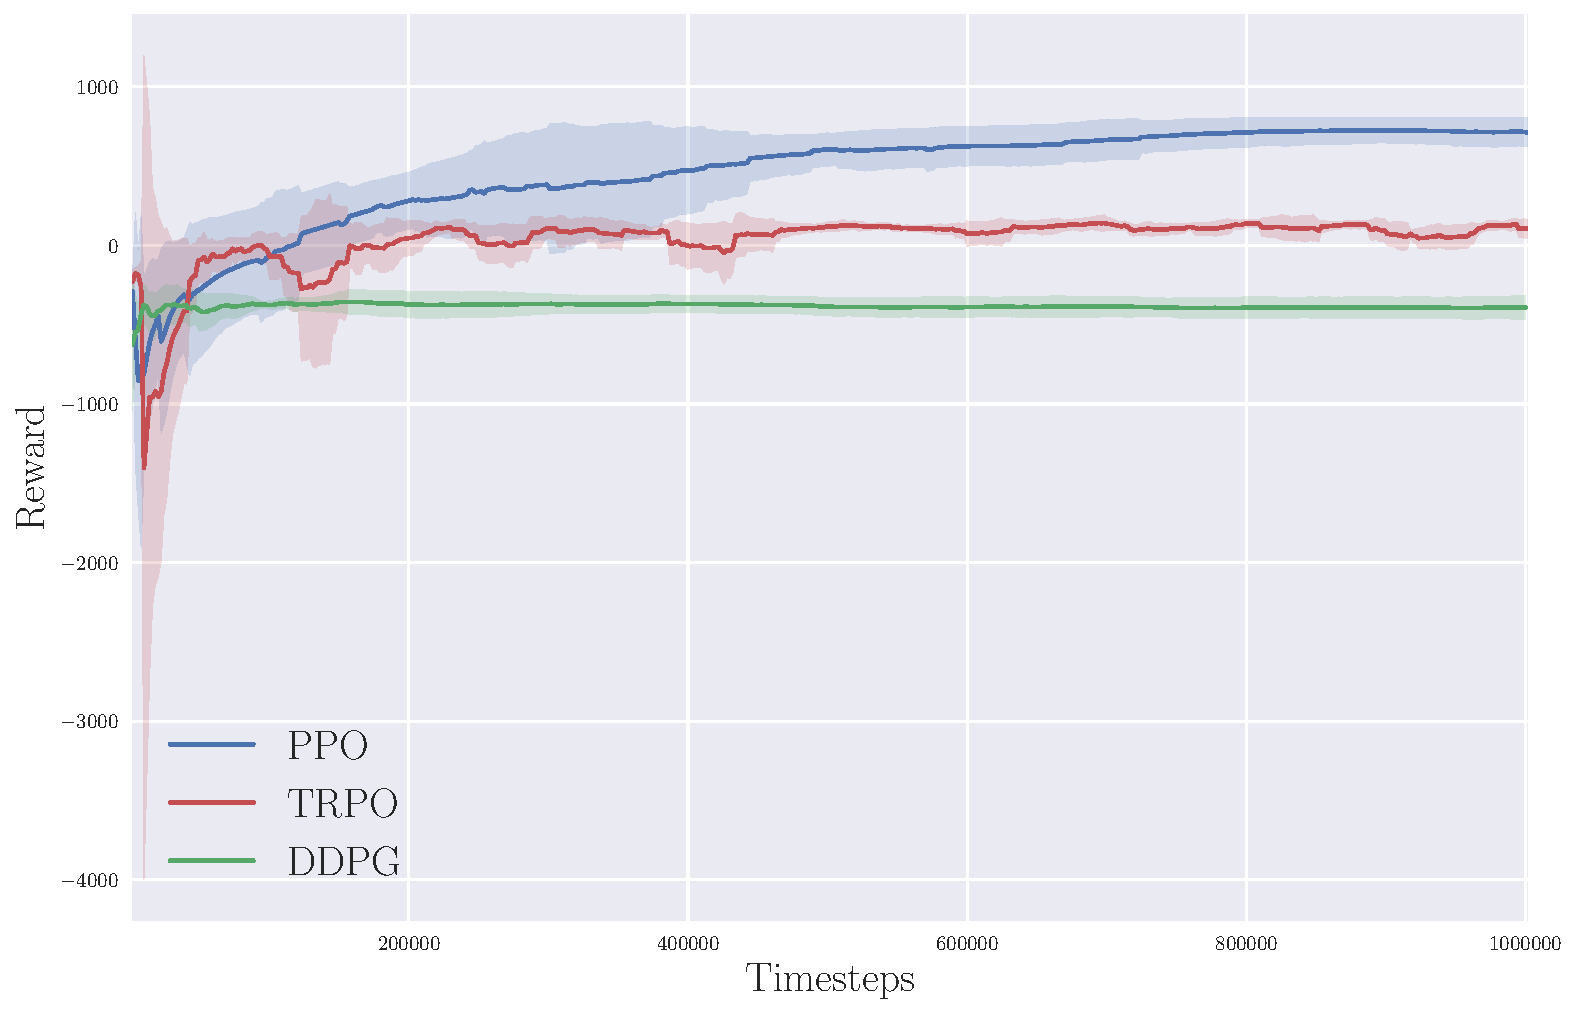
\includegraphics[width=0.9\textwidth]{Chapter7/reward.pdf}
	\caption{Average reward for PPO, TRPO and DDPG in the Racer task during training.
	The dark line is the mean over the $5$ runs and the transparent filling is
	 the standard deviation in regards to the mean.}
	\label{fig:racer_episode_rew}
\end{figure}

\begin{figure}[ht]
	\centering
	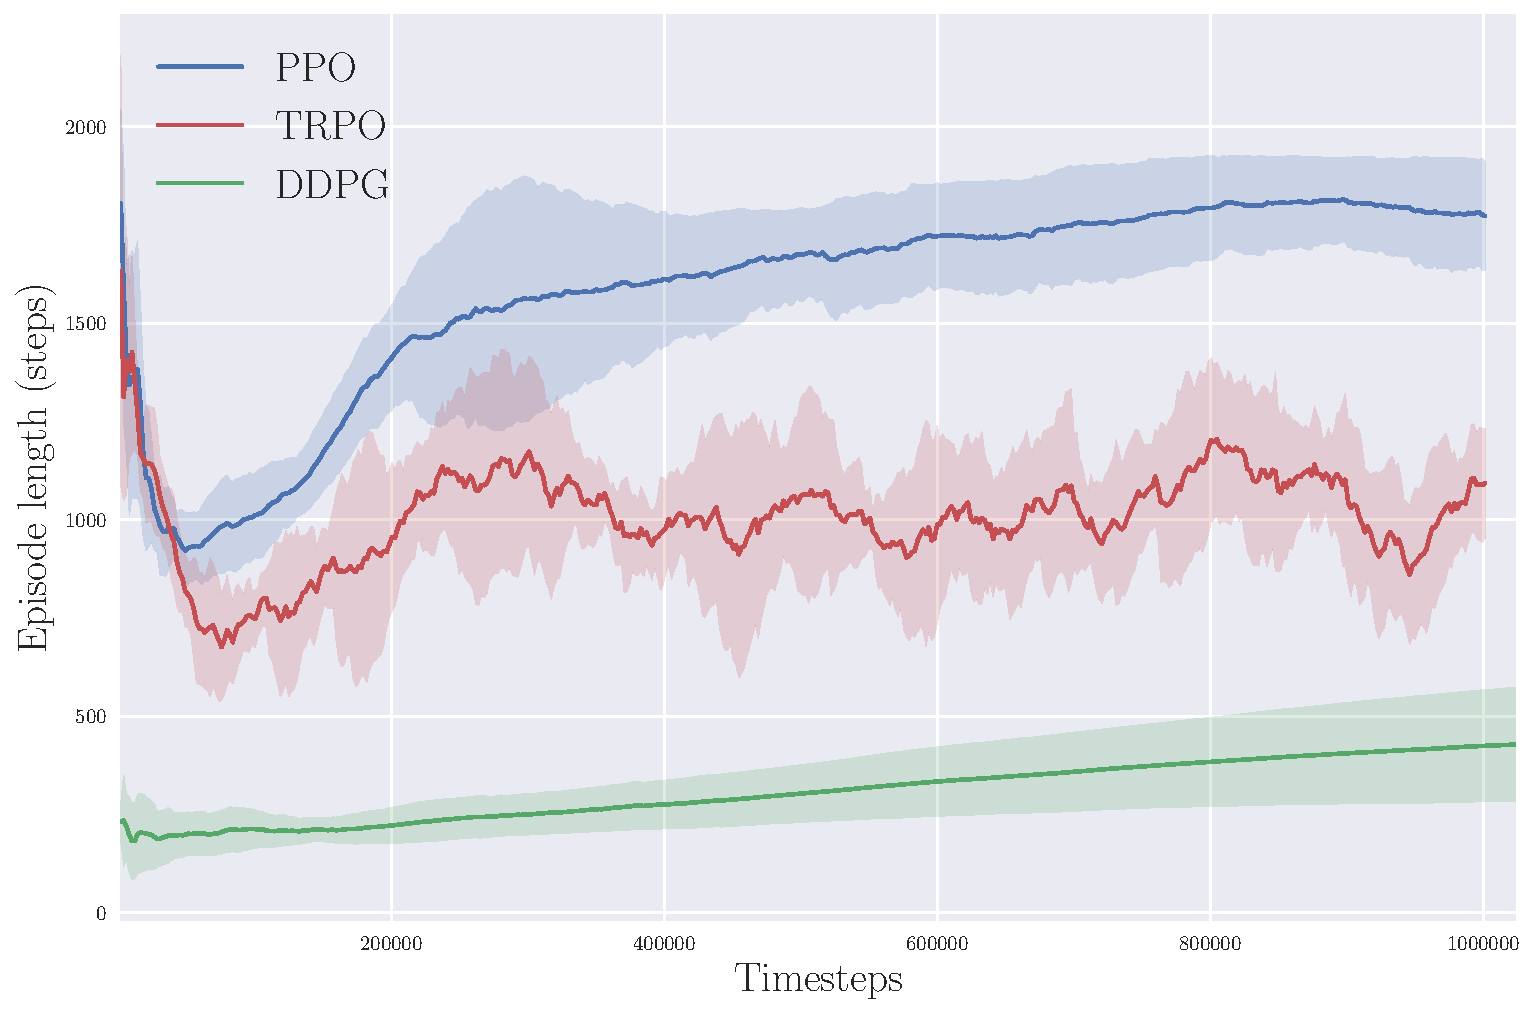
\includegraphics[width=0.9\textwidth]{Chapter7/episode_length.pdf}
	\caption{Episode length for PPO, TRPO and DDPG in the Racer task during training.
	The dark line is the mean over the $5$ runs and the transparent filling is
	the standard deviation in regards to the mean.}
	\label{fig:racer_episode_len}
\end{figure}

Figures and \ref{fig:racer_episode_rew} and \ref{fig:racer_episode_len} clearly show that 
the performance of PPO is consistently better than DDPG and TRPO for the racer task.
It is important to note that in the first $200000$ timesteps, the episode length for PPO and
TRPO are below the episode length at the end of training.
This means that, initially, that the robot is constantly falling down or leaving the race track until
it starts to learn that a better policy is to avoid falling and to stay on track, so the episodes
progressively take longer to terminate.
We also point out that the DDPG agent barely improves over time.

During the evaluation phase, we observe that the only agent that actually reaches the finish line was the 
robot trained using PPO. 
We chose one of the learned policies and used it to compare against an open loop ``go-straight" controller
that simply goes straight.
We analyse 20 trajectories executed by the PPO learned policy and compare them with those executed by the baseline.
The results are show in Figure \ref{fig:trajectory}.

\begin{figure}[b]
	\centering
	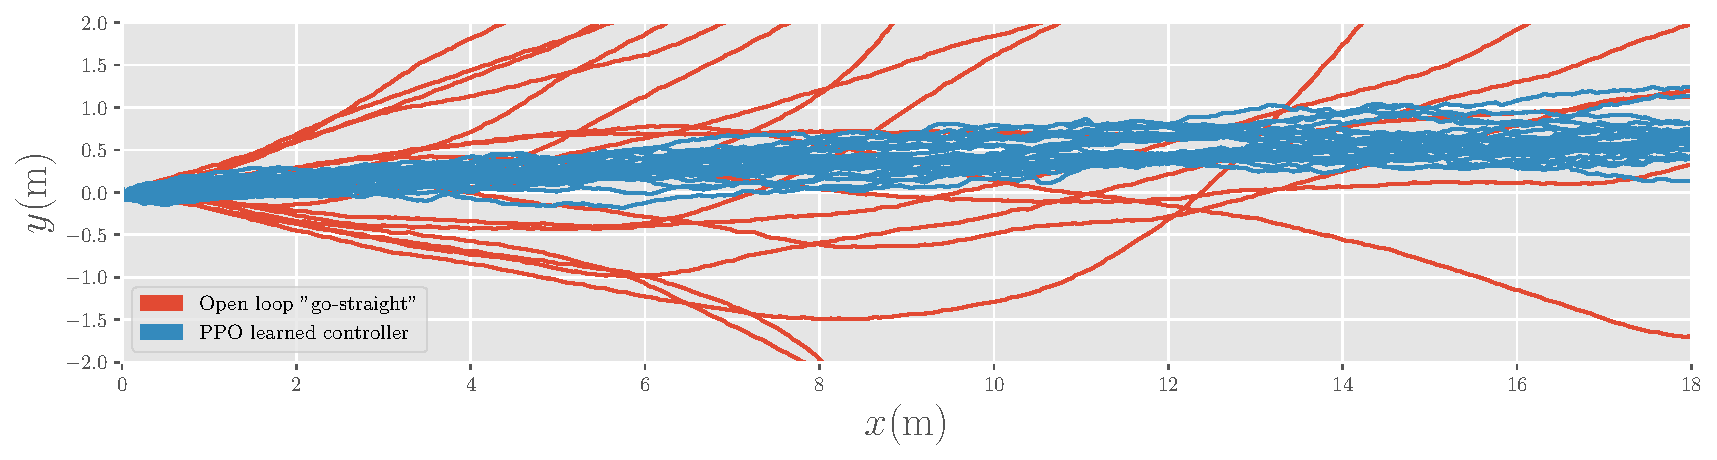
\includegraphics[width=1\textwidth]{Chapter7/trajectory.pdf}
	\caption{Trajectories comparison between one of the trained PPO controllers and the open loop ``go-straight" controller.}
	\label{fig:trajectory}
\end{figure}

For these trajectories, the empirical results can be summarized as follows: 

\begin{itemize}
	\item \textbf{Total race average speed} $\overline{v_x} \approx 0.6$ m/s. The speed expresses how fast, on average,
	the agent completed the race. Notice that the walking engine's stability constraints limits the robot's
	speed to approximately $0.9$ m/s. Therefore, in comparison to both the baseline - that rarely finishes the task - and
	theoretical fastest policy, the learned policy does very well on this task.
	\item \textbf{Horizontal displacement average} $y_{\text{mean}} \approx 0.47$ m. This represents how far,
	horizontally, from to the center line of the race track, the agent finishes the race. Since the race track
	is 4m wide, the average horizontal displacement is small as shown in Figure \ref{fig:trajectory}.
	Note that the robot did not leave the race track in all $20$ trajectories.
\end{itemize}

These results show that the robot successfully learned how to complete the task, performing significantly better
than the baseline.
However, we also observe that this policy was a bit biased in regards to the horizontal displacement
and therefore could still be further improved.

\section{Humanoid Soccer Dribbling Task}

In this problem, we ran PPO, TRPO and DDPG during $1.7\text{x} 10^6$ timesteps with the parameters described in Appendix
\ref{chap:appendix_experiment}. In comparison with the other tasks, learning to dribble
requires much more data since it is a far more challenging task.
We compare the performance of these algorithms and analyse how well the learned policy does in comparison to
the baseline dribble behavior implemented by the ITAndroids team.
On average, each experiment took much longer to run, around $8$ hours per experiment.
The main reason for this is that there is an additional simulation robot that
interacts with the environment. 
This was very challenging, since this made the process of iterating over different approaches much slower.

Similarly to the previous task, 
we ran the experiments $5$ times for each algorithm and calculated the performance mean and standard deviation over all runs.
Figure \ref{fig:dribbling_episode_rew} depicts the episode rewards during the training phase for all runs. 
The dark line represents the reward mean and the transparent filling is the standard deviation
of all the executions.

\begin{figure}[h]
	\centering
	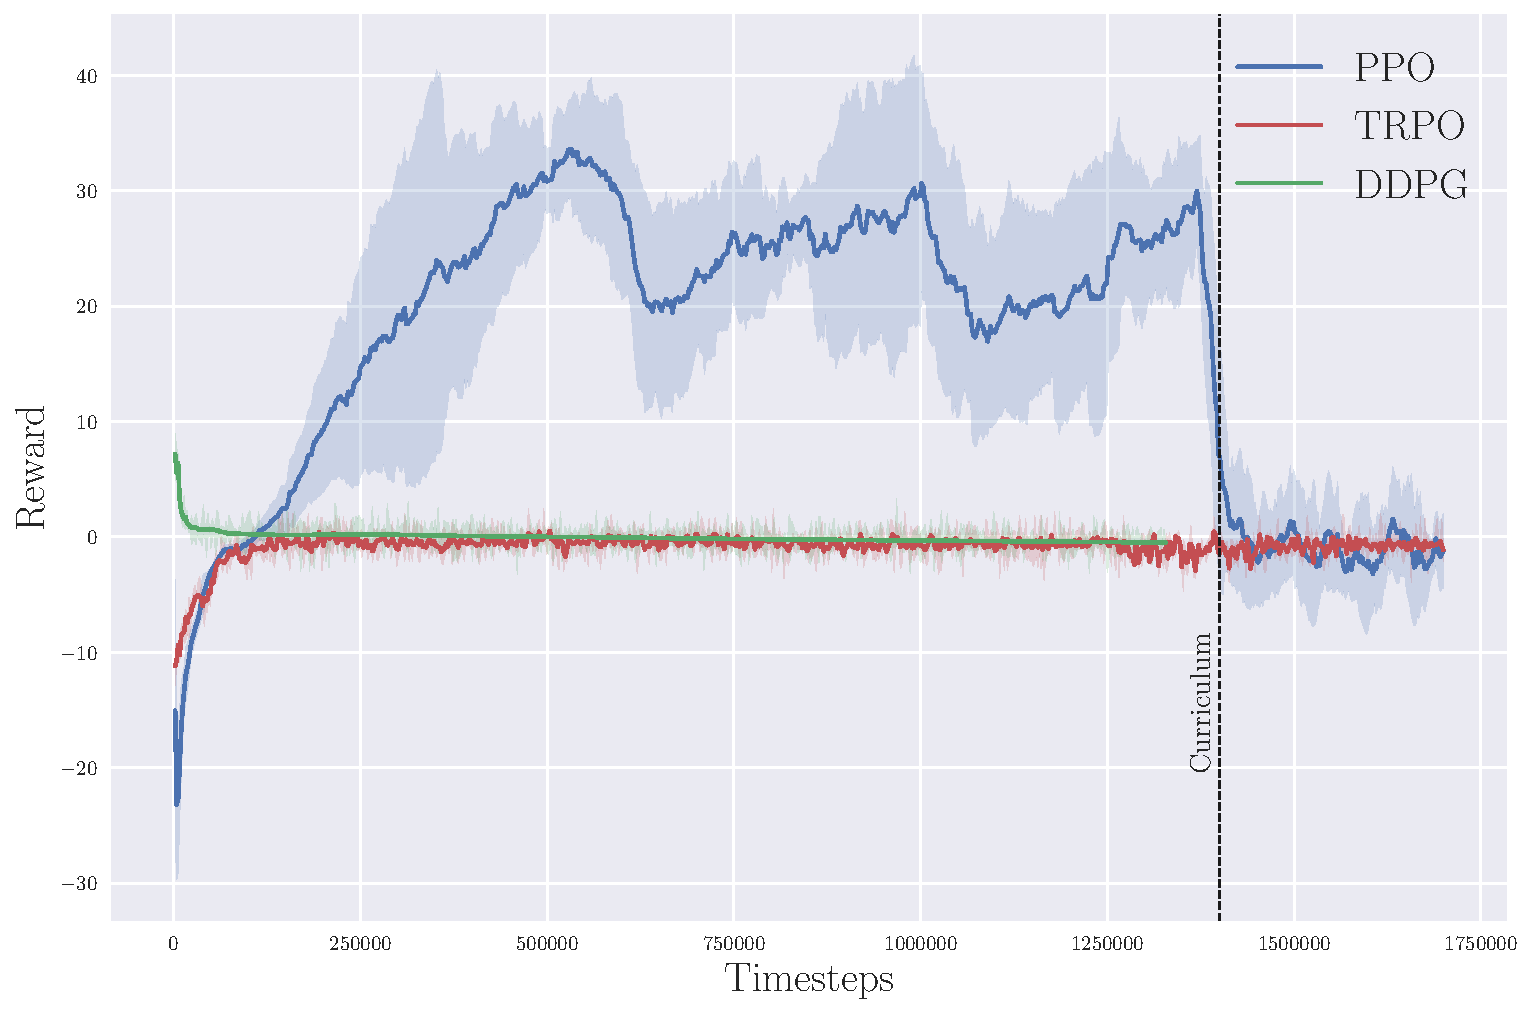
\includegraphics[width=0.9\textwidth]{Chapter7/dribbling/Reward.pdf}
	\caption{Average reward for PPO, TRPO and DDPG in the dribbling task during training.
	The dark line is the mean over the $5$ runs and the transparent filling is
	 the standard deviation in regards to the mean and the doted line represents when the curriculum changes.}
	\label{fig:dribbling_episode_rew}
\end{figure}

For PPO, we notice a sharp drop in the average reward when the curriculum changes.
This is expected since a better opponent makes it harder for the learning agent to complete the dribble
(and get more reward). Furthermore, not all agents are able to successfully learn to dribble since the 
average rewards for some agents are negative.
Similarly, Figure \ref{fig:dribbling_episode_len} illustrates episode length mean $\pm$ the standard deviation
over the same five runs.

\begin{figure}[h]
	\centering
	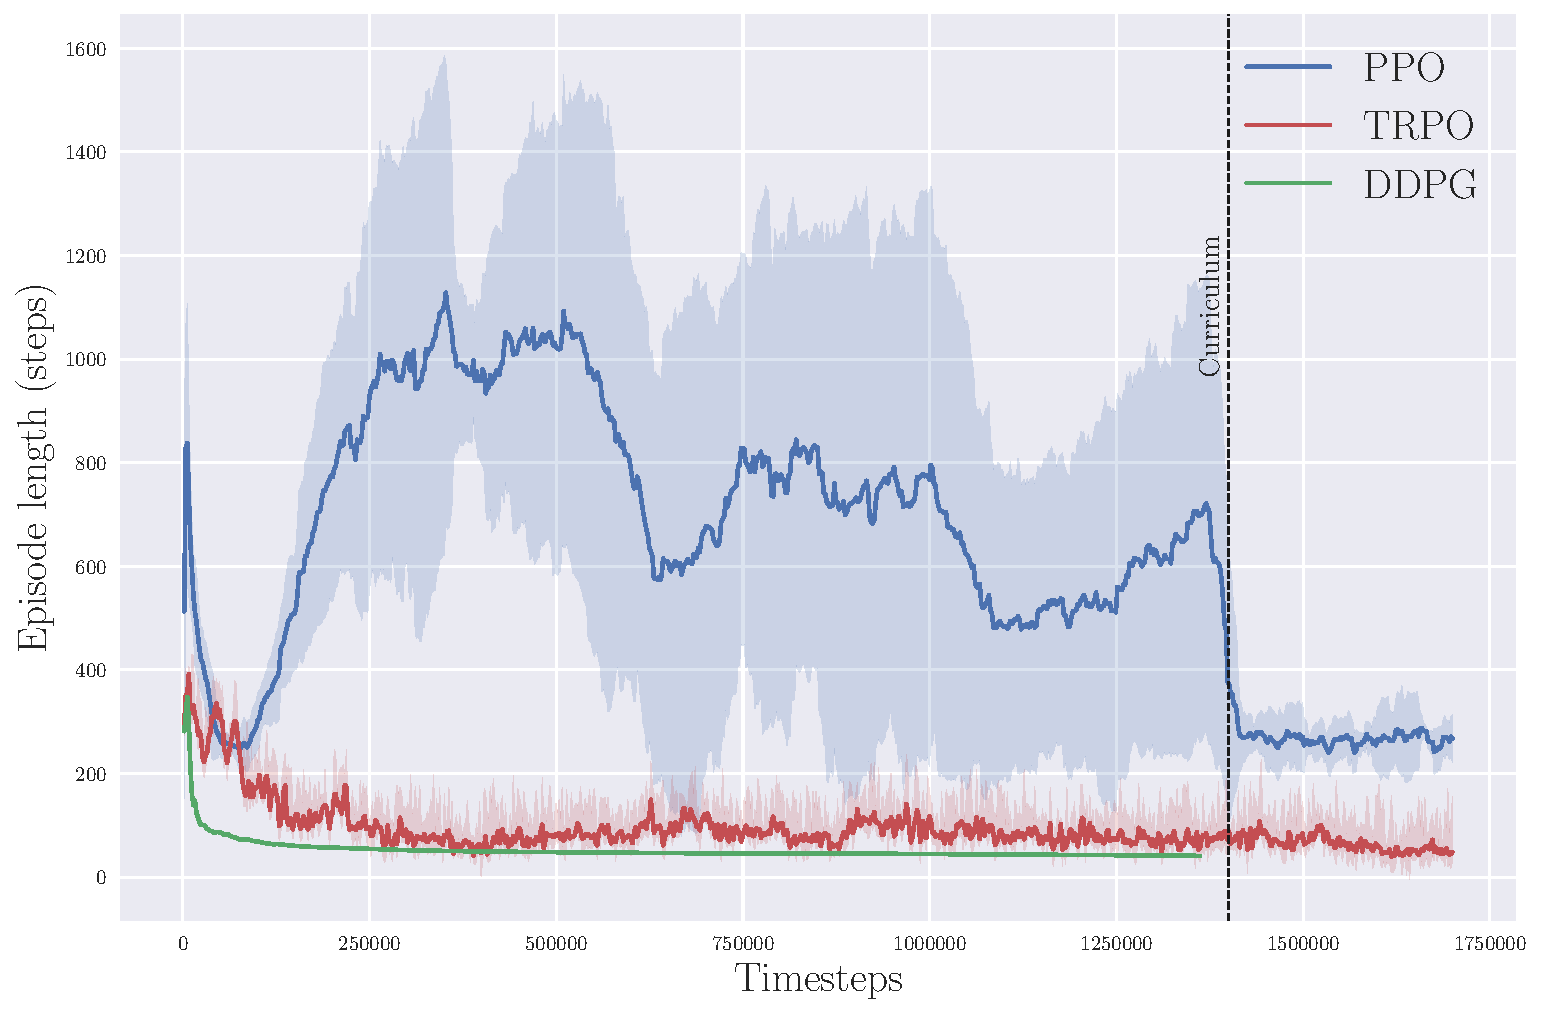
\includegraphics[width=0.9\textwidth]{Chapter7/dribbling/Episodelength(steps).pdf}
	\caption{Episode length for PPO, TRPO and DDPG in the dribbling task during training.
	The dark line is the mean over the $5$ runs and the transparent filling is
	the standard deviation in regards to the mean and the doted line represents when the curriculum changes.}
	\label{fig:dribbling_episode_len}
\end{figure}

We notice a similar sharp drop in the episode duration when the curriculum changes. This is also
expected since the agent must learn to dribble faster to avoid losing the ball to the opponent.
Furthermore, the average reward has a higher variance in comparison to the previous task.
This could mean that the policy space of successful dribbling policies is higher than for the
previous task since the task is significantly more complex.

% Figures and \ref{fig:racer_episode_rew} and \ref{fig:racer_episode_len} clearly show that 
% the performance of PPO is consistently better than DDPG and TRPO for the racer task.
% It is important to note that in the first $200000$ timesteps, the episode length for PPO and
% TRPO are below the episode length at the end of training.
% This means that, initially, that the robot is constantly falling down or leaving the race track until
% it starts to learn that a better policy is to avoid falling and staying on track and the episodes
% progressively take longer to terminate.
% We also point out that the DDPG agent barely improves over time.

To evaluate our results, we chose one of the learned policies and ran this task for $2000$ episodes
against the ITAndroids baseline agent.
We used metric $M$ for measuring how good the agent performed on the task and is given by the rate of successful dribbles,
defined in Equation \ref{eq:metric}.

\begin{equation}
	M = \dfrac{N_{\text{agent dribbles}}}{N_{\text{agent dribbles}} + N_{\text{opp dribbles}}}
	\label{eq:metric}
\end{equation}
where $N_{\text{agent dribbles}}$ is the number of successful dribbles by the agent and
$N_{\text{agent dribbles}}$ is number of successful dribbles by the opponent.
We considered a successful dribble when an agent managed to move the ball
out of the task region, towards its attacking side.
We also calculated how long, on average, each robot takes to complete the dribble.

The results are summarized in Table \ref{tab:dribble}

\begin{table}[ht]
    \begin{tabular}{|l|l|l|}
    \hline
    Agent            &Successful dribble rate ($M$)   & Average dribble duration (in timesteps) \\ \hline
    Learning Agent   &$ 68.2$\%                       & $298.2$               \\
    Baseline Agent   &$ 31.8$\%                       & $321.6$                \\ \hline
    \end{tabular}
\centering
\caption{Evaluation results of the dribbling task.}
\label{tab:dribble}
\end{table}

We can see that the learned agent greatly outperforms the baseline, despite taking longer on average
to complete the task.
A video of the trained agent executing the task is available at the GitHub repository.


% REFERENCIAS BIBLIOGRAFICAS
\renewcommand\bibname{\itareferencesnamebabel} %renomear titulo do capitulo referencias
\bibliography{Referencias/referencias}

% Apendices
%\appendix
%\chapter{Topicos de Dilema Linear} %opcional
%\section{Uma Primeira Se��o para o Ap�ndice}

A matriz de Dilema Linear $M$ e o vetor de torques inerciais $b$,
utilizados na simula��o s�o calculados segundo a formula��o 
abaixo:
\begin{equation}
M=\left[ \begin{array}{ccc}
M_{11} & M_{12} & M_{13} \\
M_{21} & M_{22} & M_{23} \\
M_{31} & M_{32} & M_{33}
\end{array} \right]
\end{equation}

\begin{figure}[h]
\centering
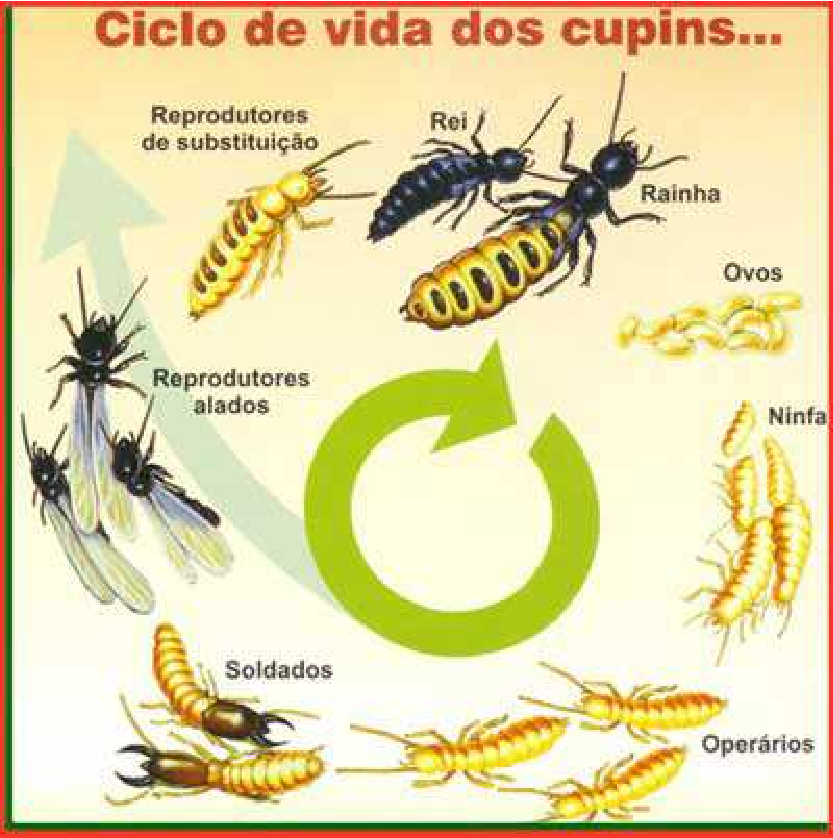
\includegraphics[height=5cm, width=5cm]{ApeA/pragas_ciclo_cupim}
\caption{Uma figura que est� no ap�ndice}\label{FD}
\end{figure}


% Anexos
%\annex
%\chapter{Exemplo de um Primeiro Anexo} %opcional
%% Texto do Primeiro Anexo
\section{Uma Se��o do Primeiro Anexo}
% Texto da primeira secao do primeiro anexo
Algum texto na primeira se��o do primeiro anexo.



% Glossario
%\itaglossary
%\printglossary

% Folha de Registro do Documento
% Valores dos campos do formulario
\FRDitadata{29 de JUnho de 2018}
\FRDitadocnro{DCTA/ITA/DM-018/2015} %(o numero de registro voce solicita a biblioteca)
\FRDitaorgaointerno{Instituto Tecnol\'ogico de Aeron\'autica -- ITA}
%Exemplo no caso de pos-graduacao: Instituto Tecnol{\'o}gico de Aeron{\'a}utica -- ITA
\FRDitapalavrasautor{Din\^amica de rob\^os; Rob\^os human\'oides; Controle de rob\^os; Intelig\^encia artificial; Rob\'otica; Controle}
\FRDitapalavrasresult{Din\^amica de rob\^os; Rob\^os human\'oides; Controle de rob\^os; Intelig\^encia artificial; Rob\'otica; Controle}
%Exemplo no caso de graduacao (TG):
%\FRDitapalavraapresentacao{Trabalho de Graduacao, ITA, Sao Jose dos Campos, 2015. \NumPenultimaPagina\ paginas.}
%Exemplo no caso de pos-graduacao (msc, dsc):
\FRDitapalavraapresentacao{ITA, S\~ao Jos\'e dos Campos. Curso de Gradua\c c\~ao em Engenharia Eletr\^onica. \'area de Ci\^encia da Computa\c c\~ao. Orientador: Prof.~Dr. Marcos Ricardo Omena de A. M\'aximo. Coorientador: Prof.~Dr. Takashi Yoneyama. Defesa em 21/11/2018. }
\FRDitaresumo{

%Futebol de robôs humanoides é uma atividade bem competitiva que visa ampliar os limites da pesquisa em robótica. Um dos diversos desafios envolvidos em jogar futebol é o desafio de chutar a bola eficientemente, de acordo com cada situação ao longo da partida. Além disso, temos presenciado um avanço continuo nas técnicas recentes em Deep Reinforcement Learning para aprender complexos problemas de controle em espaços de estados contínuo, como problemas de locomoção e de diversos movimentos presentes em robótica. DRL livre de modelo é um campo da grande área de aprendizado de máquina que combina algoritmos de aprendizado por reforço (RL) com métodos de aprendizado supervisionado (SL) utilizando deep neural-networks. DRL se adequa muito bem a problemas de locomoção em robótica, uma vez que elimina a necessidade de modelar a complexa dinâmica de um robô humanoide. Nesse trabalho, nós focamos no específico problema de ensinar um robô humanoide a chutar uma bola em direção a uma distância final planejada. Primeiramente, esse documento apresenta uma descrição do problema, acompanhada dos trabalhos relacionados e da abordagem proposta pelos autores, em seguida, é fornecida uma introdução às teorias relacionadas a aprendizado por reforço e a aprendizado supervisionado, finalizando com uma descrição sucinta das técnicas mais recentes em DRL. No futuro, planejamos alcançar um comportamento completo na ação mencionada, através do uso de algoritmos em DRL para inicialmente aprender um comportamento básico a partir da imitação de um movimento de chute existente, e então desenvolver o comportamento de forma aprender por reforço a chutar a bola até uma distância final desejada.

%Humanoid robot soccer is a very traditional competitive task that aims to push boundaries of state-of-the-art in robotics. One of the many challenges of playing soccer is kicking a ball efficiently, according to each context during the game. Besides, we have been witnessing the improvement in modern Deep Reinforcement Learning (DRL) techniques towards the goal of learning complex continuous control problems such as locomotion and several others movements present in robotics. Model-free DRL is a Machine-Learning field that combines Deep Learning (DL) methods with Reinforcement Learning (RL) algorithms, and greatly fit robotics locomotion problems since it avoids dealing with complex dynamics of a humanoid robot. In this work, we focused on a particular problem of the humanoid robot soccer domain which consists in teaching the robot to kick a ball towards a final planned distance. This document first gives a presentation of the given problem, with the related works and proposed approach, followed by a introduction of some background concerning RL and DL, ending with a summarized description of some cutting-edge DRL techniques. In the future, we plan to achieve a full behavior for the intended action, by using DRL techniques in first learning a initial behavior, using imitation learning on an already built kick movement, and then learning how to achieve the ultimate goal of reaching a desired final distance for the ball.}
%  Primeiro Parametro: Nacional ou Internacional -- N/I
%  Segundo parametro: Ostensivo, Reservado, Confidencial ou Secreto -- O/R/C/S
\FRDitaOpcoes{N}{O}
% Cria o formulario
\itaFRD

\end{document}
% Fim do Documento. O massacre acabou!!! :-)
